\documentclass[11pt]{article}

\usepackage{
    amssymb,
    amsmath,
    amsfonts,
    calc,
    eurosym,
    geometry,
    ulem,
    graphicx,
    caption,
    color,
    setspace,
    sectsty,
    comment,
    footmisc,
    caption,
    % natbib,
    pdflscape,
    subcaption,
    subfiles,
    titling,
    array,
    hyperref,
    booktabs,
    longtable,
    float,
    authblk,
    makecell,
    threeparttable,
    pgfplots}

\usepackage[page]{appendix} % print appendices title

\usepackage[
    backend=biber,
    style=nature,
    date=year,
    doi=true,
    isbn=false,
    url=false,
    eprint=false
]{biblatex}



\AtEveryBibitem{%
  \clearfield{note}%
}
\AtEveryCitekey{\clearlist{publisher}}
\AtEveryBibitem{\clearlist{publisher}}

\usepackage{pgf,tikz}
\usetikzlibrary{arrows, automata}
\usetikzlibrary{shapes.geometric}
\usetikzlibrary{positioning,calc, decorations.pathreplacing}

\usepackage{siunitx}
\newcolumntype{d}{S[input-symbols = ()]}

\normalem

\renewcommand\Affilfont{\small\itshape}

\onehalfspacing
\newtheorem{theorem}{Theorem}
\newtheorem{corollary}[theorem]{Corollary}
\newtheorem{proposition}{Proposition}
\newenvironment{proof}[1][Proof]{\noindent\textbf{#1.} }{\ \rule{0.5em}{0.5em}}

\newtheorem{hyp}{Hypothesis}
\newtheorem{subhyp}{Hypothesis}[hyp]
\renewcommand{\thesubhyp}{\thehyp\alph{subhyp}}

\newcommand{\red}[1]{{\color{red} #1}}
\newcommand{\blue}[1]{{\color{blue} #1}}

\newcolumntype{L}[1]{>{\raggedright\arraybackslash}m{#1}}
\newcolumntype{C}[1]{>{\centering\arraybackslash}m{#1}}
\newcolumntype{R}[1]{>{\raggedleft\arraybackslash}m{#1}}
\subsubsectionfont{\normalfont\itshape}

\usepackage{mathtools}

\usepackage{letltxmacro}
\LetLtxMacro\orgvdots\vdots
\LetLtxMacro\orgddots\ddots

\makeatletter
\DeclareRobustCommand\vdots{%
  \mathpalette\@vdots{}%
}
\newcommand*{\@vdots}[2]{%
  % #1: math style
  % #2: unused
  \sbox0{$#1\cdotp\cdotp\cdotp\m@th$}%
  \sbox2{$#1.\m@th$}%
  \vbox{%
    \dimen@=\wd0 %
    \advance\dimen@ -3\ht2 %
    \kern.5\dimen@
    % remove side bearings
    \dimen@=\wd2 %
    \advance\dimen@ -\ht2 %
    \dimen2=\wd0 %
    \advance\dimen2 -\dimen@
    \vbox to \dimen2{%
      \offinterlineskip
      \copy2 \vfill\copy2 \vfill\copy2 %
    }%
  }%
}
\DeclareRobustCommand\ddots{%
  \mathinner{%
    \mathpalette\@ddots{}%
    \mkern\thinmuskip
  }%
}
\newcommand*{\@ddots}[2]{%
  % #1: math style
  % #2: unused
  \sbox0{$#1\cdotp\cdotp\cdotp\m@th$}%
  \sbox2{$#1.\m@th$}%
  \vbox{%
    \dimen@=\wd0 %
    \advance\dimen@ -3\ht2 %
    \kern.5\dimen@
    % remove side bearings
    \dimen@=\wd2 %
    \advance\dimen@ -\ht2 %
    \dimen2=\wd0 %
    \advance\dimen2 -\dimen@
    \vbox to \dimen2{%
      \offinterlineskip
      \hbox{$#1\mathpunct{.}\m@th$}%
      \vfill
      \hbox{$#1\mathpunct{\kern\wd2}\mathpunct{.}\m@th$}%
      \vfill
      \hbox{$#1\mathpunct{\kern\wd2}\mathpunct{\kern\wd2}\mathpunct{.}\m@th$}%
    }%
  }%
}
\makeatother

\pgfmathdeclarefunction{gauss}{2}{%
  \pgfmathparse{1/(#2*sqrt(2*pi))*exp(-((x-#1)^2)/(2*#2^2))}%
}

\pgfmathdeclarefunction{lnormal}{2}{%
  \pgfmathparse{1/(x*#2*sqrt(2*pi))*exp(-((ln(x)-#1)^2)/(2*#2^2))}%
}

\pgfmathdeclarefunction{poisson}{1}{%
\pgfmathparse{(#1^x)*exp(-#1)/(x!)}
}

% \pgfmathdeclarefunction{gammapdf}{2}{
% \pgfmathparse{1/(#2^#1*gamma(#1))*x^(#1-1)*exp(-x/#2)}
% }

\usepgfplotslibrary{fillbetween}

\geometry{left=1.0in,right=1.0in,top=1.0in,bottom=1.0in}

\addbibresource{pep.bib}

\begin{document}

\begin{titlepage}
\title{Defining and emulating target trials of the effects of postexposure vaccination using observational data}
\author[1]{Christopher Boyer\thanks{email: \href{mailto:cboyer@hsph.harvard.edu}{cboyer@hsph.harvard.edu}}}
\author[1]{Marc Lipsitch}
\affil[1]{Department of Epidemiology, Harvard T.H. Chan School of Public Health, Boston, MA.}
\date{\today}
\maketitle

\begin{abstract}
Postexposure vaccination has the potential to prevent or modify the course of clinical disease among those exposed to a pathogen. However, due to logistical constraints, postexposure vaccine trials have been difficult to implement in practice. In place of trials, investigators have used observational data to estimate the efficacy or optimal timing window for postexposure vaccines, but the relationship between these analyses and those that would be conducted in a trial is often unclear. Here, we define several possible target trials for postexposure vaccination and show how, under certain conditions, they can be emulated using observational data. We emphasize the importance of the incubation period and the timing of vaccination in trial design and emulation. As an example, we specify a protocol for postexposure vaccination against mpox and provide a step-by-step description of how to emulate it using data from a healthcare database or contact tracing program. We further illustrate some of the benefits of the target trial approach through simulation.
\noindent \\
\vspace{0in} \\
\noindent\textbf{Keywords:} target trial, vaccines, immortal time bias, effectiveness, monkeypox, postexposure prophylaxis, infectious disease \\

\bigskip
\end{abstract}
\setcounter{page}{0}
\thispagestyle{empty}
\end{titlepage}
\pagebreak \newpage

\doublespacing


\section{Introduction} \label{sec:introduction}
For a millenium or more humans have been inoculating healthy, unexposed individuals to prevent the onset of future disease \cite{plotkin2012vaccines}. Today, this remains the dominant paradigm for the development and mass administration of vaccines. By contrast, using vaccines to prevent clinical disease among those \textit{already exposed} to a pathogen, i.e. postexposure vaccination, remains an under-utilized strategy despite its potential to curb outbreaks and prevent the worst sequelae of disease \cite{gallagher_postexposure_2019}. This is due, in part, to the difficulty of running postexposure trials to establish vaccine efficacy, particularly during a larger outbreak. In these trials investigators must identify, randomize, and vaccinate participants all in the time window between exposure and symptom onset. Depending on the pathogen, this window can be incredibly compressed ---on the order of a few days to a week. Furthermore, vaccine effectiveness may be highly dependent upon the the time since exposure. Thus, even when trials are possible it can be difficult to compare effectiveness estimates across trials with different distributions of vaccination times or to infer an optimal postexposure window in which to vaccinate. Moreover, when there is other evidence to support effectiveness, for instance from pre-exposure trials or immunogenecity studies, and when other treatments are unavailable, a randomized postexposure trial may be considered unethical.

In absence of trial data, an alternative approach is to use observational data to emulate the trial desired \cite{hernan_observational_2008,hernan_using_2016} (called a "target trial"), for instance by using electronic healthcare records from a large healthcare system or other passive surveillance systems, or by using public health contact tracing databases to define cohorts of individuals exposed to infection and comparing outcomes among those who do and do not receive post-exposure vaccination. In this paper, we define several target trials for assessing the effectiveness of postexposure vaccination depending on the causal quantity of interest. We also discuss the conditions under which such a trial can be emulated from observational data. We show how adopting a target trial framework can help clarify the causal question and resolve common biases in the analysis of postexposure efficacy using observational data through alignment of time zero, eligibility, and assignment as well as unambiguous definition of the treatment strategies being contrasted. We provide an example protocol for emulating a trial of a postexposure vaccine for mpox and illustrate some of the benefits of this approach through simulation.

\section{Design challenges: incubation period and timing of vaccination}
Both the design of postexposure trials and attempts to emulate them using observational data are complicated by the interaction between the incubation period of the pathogen and the postexposure timing of vaccination. To provide benefit postexposure, a vaccine must stimulate an immune response faster, greater, or more specific than that provoked by natural infection alone. For example, in the case of smallpox, a vaccine administered within 72 hours after exposure to variola virus (the causative virus of smallpox) induces an antibody response 4 to 8 days earlier than the variola virus itself, most likely because the vaccine response bypasses the initial stages of natural infection in the respiratory tract, and thereby can prevent the onset of clinical disease \cite{massoudi_effectiveness_2003,keckler_effects_2013}. However, postexposure delays in receiving the vaccine, within certain limits, are often outside the control of investigators, as participants must first be notified of their exposure and present at a healthcare clinic prior to receiving a vaccine. 

The resulting overlap between the timing of vaccination and the timing of symptom onset creates several design challenges (see Figure \ref{fig:illustration1}). First, the effectiveness of a vaccine may vary substantially depending on how quickly participants can be vaccinated postexposure (top panel, Figure \ref{fig:illustration1}). In a randomized trial, a trialist must strike a balance between specifying a realistic protocol for vaccination timing that takes into account existing exposure identification, enrollment, and care coordination systems with what is known about the biology governing the clinical course of infection and the vaccine's ability to pre-empt it. This can be difficult when the incubation period or mechanism of action of a postexposure vaccine are not well established. Under these circumstances, longer delays may be permitted with a secondary goal to infer the optimal postexposure window to administer the vaccine. In an observational setting, by contrast, the protocol for vaccine timing is often less clear or may even be absent, in which case the vaccination strategy being evaluated may be ambiguous.

Second, when vaccination is delayed there is also the possibility that some participants may have already developed symptoms prior to enrollment or vaccination, particularly when there is substantial overlap between referral or administration times and the incubation period. In order for a vaccine to fully prevent symptom onset, logically it should be administered prior to the development of symptoms. However, when those who have symptoms at enrollment are excluded, this has implications for the population to which estimates can be generalized, as the design implicitly conditions on those who survive symptom free. When they are included, they may attenuate estimates of vaccine effectiveness relative to an ideally conducted trial as presumably vaccination post symptom onset is ineffective at preventing illness. 

Finally, a challenge specific to observational studies is the lack of an unambiguous assignment to a treatment strategy at time zero \cite{hernan_how_2018}. In a trial, participants are explicitly assigned to either vaccine or no vaccine (or placebo) at the time of enrollment and prospectively followed. By contrast, in an observational study, exposure is often defined retrospectively by what participants do over the follow up period (middle panel, Figure \ref{fig:illustration1}). Depending on how this is handled, the ambiguity in assignment coupled with delay in receiving vaccines creates the possibility of bias due to \textit{immortal time} among the vaccinated as they have to survive symptom-free long enough to become vaccinated \cite{suissa_immortal_2008}, whereas the unvaccinated may be defined independently of their survival time. In this scenario, the vaccinated are more likely to be lower risk contacts or those who may have failed to develop symptoms in the absence of vaccination anyway. 

In a trial, the challenges posed by overlapping delays in vaccination and symptom onset can be addressed through careful design and a clear protocol, for instance by specifying a  window in which people can be vaccinated, by stratifying on enrollment date, and by clear eligibility criteria. In an observational study, these fixes are often unavailable to investigators at the design stage. However, we argue that, many challenges can still be resolved by specifying the target trial that one would like to perform, but can't, and attempting to emulate it using the observational data (bottom panel, Figure \ref{fig:illustration1}).

\begin{figure}[p]
    \centering
    \begin{tikzpicture}
        \begin{axis}[
          no markers, domain=0:15, samples=100,
          axis lines*=left, xlabel=day, ylabel=$ $,
          title={Symptom onset times},
          height=5.5cm, width=15cm,
          xtick={1,2,3,4,5,6,7,8,9,10,11,12,13,14,15}, ytick=\empty,
          enlargelimits=false, clip=false, axis on top,
          grid = none, name=onset
          ]
          \addplot [draw=none, fill=blue!20] {lnormal(1.75,0.33)}\closedcycle;
          \addplot [very thick, blue!50!black] {lnormal(1.75,0.33)};
        %   \addplot [draw=none, fill=orange!20] {gammapdf(4, 1)}\closedcycle;
        %   \addplot [very thick, orange!50!black] {gammapdf(4, 1)};
          \addplot [very thick, red] {0.222 / (1 + exp(0.9 * (x - 4)))};
          \node[red] at (axis cs: 2.65,0.2) {$VE(t)$};
        \end{axis}
        \begin{axis}[
          at=(onset.below south west),
          anchor=north west,
          yshift=-1.3cm,
          domain=0:15, samples=100,
          axis lines*=left, xlabel=$\text{day}$, ylabel=$ $,
          title={Observational study},
          height=5.5cm, width=15cm, ymin=0, ymax=13,
          xtick={1,2,3,4,5,6,7,8,9,10,11,12,13,14,15}, ytick=\empty,
          enlargelimits=false, clip=false, axis on top,
          grid=none, y axis line style={draw=none},name=obs
          ]
          \addplot[mark=none,line width=1.2pt,dashed]
          coordinates {(0,12)(4,12)};
          \addplot[mark=none,line width=1.2pt]
          coordinates {(4,12)(15,12)};
          \addplot[mark=none,line width=1.2pt,dashed]
          coordinates {(0,11)(1,11)};
          \addplot[mark=none,line width=1.2pt]
          coordinates {(1,11)(15,11)};
          \addplot[mark=none,line width=1.2pt,dashed]
          coordinates {(0,10)(3,10)};
          \addplot[mark=none,line width=1.2pt]
          coordinates {(3,10)(15,10)};
          \addplot[mark=none,line width=1.2pt,dashed]
          coordinates {(0,9)(2,9)};
          \addplot[mark=none,line width=1.2pt]
          coordinates {(2,9)(15,9)};
          \addplot[mark=none,line width=1.2pt,dashed]
          coordinates {(0,8)(5,8)};
          \addplot[mark=none,line width=1.2pt]
          coordinates {(5,8)(15,8)};
          
          \addplot[mark=none,line width=1.2pt]
          coordinates {(0,6)(15,6)};
          \addplot[mark=none,line width=1.2pt]
          coordinates {(0,5)(15,5)};
          \addplot[mark=none,line width=1.2pt]
          coordinates {(0,4)(15,4)};
          \addplot[mark=none,line width=1.2pt]
          coordinates {(0,3)(15,3)};
          \addplot[mark=none,line width=1.2pt]
          coordinates {(0,2)(15,2)};
          \addplot[
            mark=*,
            only marks,
            mark size=3pt
            ]
            coordinates {
            (4,12)(1,11)(3,10)(2,9)(5,8)(0,6)(0,5)(0,4)(0,3)(0,2)
          };
          \addplot[
            mark=text,
            text mark=$\boldsymbol{\times}$,
            text mark as node,
            text mark style={%
                font=\large
            },
            only marks,
            mark size=5pt
            ]
            coordinates {
            (7,8)(5,10)(2,5)(9,3)(4,4)
          };
          \node[] at (axis cs: 15.35,12) {\scriptsize V};
          \node[] at (axis cs: 15.35,11) {\scriptsize V};
          \node[] at (axis cs: 15.35,10) {\scriptsize V};
          \node[] at (axis cs: 15.35,9) {\scriptsize V};
          \node[] at (axis cs: 15.35,8) {\scriptsize V};

          \node[] at (axis cs: 15.35,6) {\scriptsize C};
          \node[] at (axis cs: 15.35,5) {\scriptsize C};
          \node[] at (axis cs: 15.35,4) {\scriptsize C};
          \node[] at (axis cs: 15.35,3) {\scriptsize C};
          \node[] at (axis cs: 15.35,2) {\scriptsize C};

        \end{axis}
        \begin{axis}[
            at=(obs.below south west),
            anchor=north west,
            yshift=-1.3cm,
            domain=0:15, samples=100,
            axis lines*=left, xlabel=$\text{day}$, ylabel=$ $,
            title={Target trial emulation},
            height=5.5cm, width=15cm, ymin=0, ymax=13,
            xtick={1,2,3,4,5,6,7,8,9,10,11,12,13,14,15}, ytick=\empty,
            enlargelimits=false, clip=false, axis on top,
            grid=none, y axis line style={draw=none}
            ]
            \addplot[mark=none,line width=1.2pt,dashed]
            coordinates {(0,12)(1,12)};
            \addplot[mark=none,line width=1.2pt]
            coordinates {(1,12)(15,12)};
            \addplot[mark=none,line width=1.2pt,dashed]
            coordinates {(0,9.75)(2,9.75)};
            \addplot[mark=none,line width=1.2pt]
            coordinates {(2,9.75)(15,9.75)};
            \addplot[mark=none,line width=1.2pt,dashed]
            coordinates {(0,7.5)(3,7.5)};
            \addplot[mark=none,line width=1.2pt]
            coordinates {(3,7.5)(15,7.5)};
            \addplot[mark=none,line width=1.2pt,dashed]
            coordinates {(0,5.25)(4,5.25)};
            \addplot[mark=none,line width=1.2pt]
            coordinates {(4,5.25)(15,5.25)};
            \addplot[mark=none,line width=1.2pt,dashed]
            coordinates {(0,3)(5,3)};
            \addplot[mark=none,line width=1.2pt]
            coordinates {(5,3)(15,3)};
            
            \addplot[mark=none,line width=1.2pt,dashed]
            coordinates {(0,11)(1,11)};
            \addplot[mark=none,line width=1.2pt]
            coordinates {(1,11)(15,11)};
            \addplot[mark=none,line width=1.2pt,dashed]
            coordinates {(0,8.75)(2,8.75)};
            \addplot[mark=none,line width=1.2pt]
            coordinates {(2,8.75)(15,8.75)};
            \addplot[mark=none,line width=1.2pt,dashed]
            coordinates {(0,6.5)(3,6.5)};
            \addplot[mark=none,line width=1.2pt]
            coordinates {(3,6.5)(15,6.5)};
            \addplot[mark=none,line width=1.2pt,dashed]
            coordinates {(0,4.25)(4,4.25)};
            \addplot[mark=none,line width=1.2pt]
            coordinates {(4,4.25)(15,4.25)};
            \addplot[mark=none,line width=1.2pt,dashed]
            coordinates {(0,2)(5,2)};
            \addplot[mark=none,line width=1.2pt]
            coordinates {(5,2)(15,2)};
            \addplot[
              mark=*,
              only marks,
              mark size=3pt
              ]
              coordinates {
              (1,12)(2,9.75)(3,7.5)(4,5.25)(5,3)(1,11)(2,8.75)(3,6.5)(4,4.25)(5,2)
            };
            \addplot[
            mark=text,
            text mark=$\boldsymbol{\times}$,
            text mark as node,
            text mark style={%
                font=\large
            },
            only marks,
            mark size=5pt
            ]
            coordinates {
            (7,3)(5,7.5)(2,11)(9,4.25)(4,8.75)
          };
            \node[] at (axis cs: 15.35,12) {\scriptsize V};
            \node[] at (axis cs: 15.35,11) {\scriptsize C};
            \node[] at (axis cs: 15.35,9.75) {\scriptsize V};
            \node[] at (axis cs: 15.35,8.75) {\scriptsize C};
            \node[] at (axis cs: 15.35,7.5) {\scriptsize V};
            \node[] at (axis cs: 15.35,6.5) {\scriptsize C};
            \node[] at (axis cs: 15.35,5.25) {\scriptsize V};
            \node[] at (axis cs: 15.35,4.25) {\scriptsize C};
            \node[] at (axis cs: 15.35,3) {\scriptsize V};
            \node[] at (axis cs: 15.35,2) {\scriptsize C};
          \end{axis}
    \end{tikzpicture}
    \caption{Illustration of the challenges of evaluating postexposure vaccination using observational data. The top panel shows the distribution of symptom onset times among cases as well as vaccine efficacy as a function of postexposure day of administration for a hypothetical pathogen. The middle panel shows an observational study with 5 vaccinated (V) and 5 unvaccinated (C) individuals in which there are delays in receiving vaccines. Dots show the time exposure status is first defined and Xs show symptom onset. The dashed line represents possible immortal time among vaccinated who have to survive symptom free long enough to be vaccinated. The bottom panel shows a nested sequence of daily trials among the same individuals in which there is no immortal time bias because the timing of enrollment and exposure assignment coincides in each trial.}
    \label{fig:illustration1}
\end{figure}


\section{Specifying the target trial}

\subsection{Set up and notation} \label{sec:setup}
We consider the emulation of a target trial designed to estimate the effect of postexposure vaccine (PEV) therapy on the $\Delta$-day risk of clinical disease. The time index $t$ denotes days since exposure to a case. We have available observational data $O=\left(L_0, A_0, D_1 \ldots, L_{\Delta-1}, A_{\Delta-1}, D_{\Delta}, X, T\right)$ on participants, where $L_t$ includes set of time-varying covariates and $L_0$ includes all covariates prior to time zero (i.e. pre-exposure). We define the following variables:
$$X: \text{ day of vaccine administration, } X = \operatorname{min}(X^*, \Delta) \text{ where } X^* \in \mathbb{N}+$$
$$T: \text{ day of clinical disease onset, } T = \operatorname{min}(T^*, \Delta) \text{ where } T^* \in \mathbb{N}+$$
$$A_t: \text{ indicator of vaccination status on day }t, A_t \in \{0, 1\}$$
$$D_t: \text{ indicator of clinical disease on day $t$, } D_t \in \{0, 1\}$$
Note that under these definitions, when $X < x$ then $A_x = 1$ and $T < \Delta$ implies $D_{\Delta} = 1$. We bin both vaccination time and symptom onset time into days since the initial exposure and censor at $\Delta$ days postexposure\footnote{i.e. those unvaccinated during follow up will have $X = \Delta$ and those without clinical disease will have $T = \Delta$}. The trial outcome $Y$ is the development of clinical disease within $\Delta$ days postexposure, i.e. $Y=D_{\Delta}$. For clarity, we make a few simplifying assumptions but discuss relaxing some of them in the appendix. First, we assume that the vaccine itself does not cause mild symptoms that can be mistaken for clinical disease. Second, we assume that the timing of the primary exposure event is measured without error and unambiguously defined. Third, we assume the goal of postexposure vaccination is the prevention of clinical disease in those exposed rather than reduction in disease severity or risk of further transmission, although in both cases the conceptualization of the target trial may be similar.

\subsection{Possible trial designs}

Under the theory that the earlier a vaccine is administered postexposure the better, the ideal causal quantity of interest, in terms of maximizing efficacy, is likely
$$VE(0) = 1 - \frac{\Pr[Y^{x = 0} = 1]}{\Pr[Y^{x > \Delta} = 1]}$$
where $Y^{x = 0}$ is a counterfactual indicator of symptoms within $\Delta$ days under \textit{immediate} postexposure vaccination on day 0 and $Y^{x > \Delta}$ is the counterfactual outcome under no vaccination over follow up\footnote{Using our definition of time-varying treatment $A_t$ we could also write this as $$VE = 1 - \frac{\Pr[Y^{\overline{a}_{\Delta} = 1} = 1]}{\Pr[Y^{\overline{a}_{\Delta} = 0} = 1]}$$}. In a randomized controlled trial with perfect adherence, this quantity could be estimated by recruiting eligible participants immediately postexposure, randomizing them to receive vaccine or no vaccine, and comparing $\Delta$-day incidence of symptoms in the two groups (We discuss estimating vaccine efficacy based on the hazard ratio rather than cumulative incidence in section \ref{sec:effect_measures} of the Appendix). 

Alternatively, if the goal was to estimate vaccine effectiveness by day, we could imagine a design in which participants are still enrolled immediately postexposure and randomized to vaccine or no vaccine, but then also randomly assigned a day that they are to receive a vaccine. In this case our casual contrast of interest is the $t$-specific vaccine efficacy
$$VE(t) = 1 - \frac{\Pr[Y^{x = t} = 1]}{\Pr[Y^{x > \Delta} = 1]}.$$
Such a design permits the estimation of the optimal day postexposure to administer a vaccine as well as the window beyond which population efficacy falls below a minimum threshold. However, several challenges prevent either of the trials mentioned above from being conducted in practice data. Chief amongst these is the fact that the timing of enrollment and vaccine administration is rarely within the control of the investigator due to delays in identifying those exposed, referring them to care, and accessing a vaccine. Even if either were feasible in a controlled environment, they would likely also be unreflective of how vaccines are actually administered in clinical practice and therefore unhelpful in informing decisions about whether to vaccinate under delays. 

When the timing of vaccination is not under the strict control of the investigator, a possible design is to specify a fixed time window in which participants are eligible to be vaccinated and randomize them on the postexposure day they present. Given that length of delay is likely a strong determinant of effectiveness, we could improve efficiency by blocking eligible participants on the postexposure day they present and performing permuted assignment to vaccine or no vaccine within enrollment-day blocks. We could then target the $t$-specific vaccine efficacy among those presenting symptom-free, i.e.
$$
VE_{T > t}(t) = 1 - \frac{\Pr[Y^{x = t} = 1 \mid X \geq t, T > t]}{\Pr[Y^{x > \Delta} = 1 \mid X \geq t, T > t]} \\
$$
by comparing vaccine and no vaccine groups within enrollment  strata. Note that, in general, the $t$-specific vaccine efficacies, $VE_{T > t}(t)$, targeted in this trial will not be the same as the $VE(t)$ defined previously as they are conditional on presentation time and being symptom-free at enrollment. Because participants are allowed to present naturally rather than being assigned a time at day zero, those that present earlier may be systematically different than those presenting later with respect to their risk of developing clinical disease. Indeed, the efficacies $VE(t)$ and $VE_{T > t}(t)$ will only coincide when there is no effect modification by enrollment day or symptom onset time. Typically, given that $VE \equiv 0$ when vaccine is administered after symptom onset, the latter condition will not be met, as $VE(t)$ will include individuals randomized to get vaccinated on a day that turns out to be after their symptom onset, while $VE_{T > t}$ does not.  Therefore, these two measures of VE answer fundamentally different questions. The first, $VE(t)$, answers the question: \textit{at the time of exposure} how effective would a vaccine be after a $t$-day delay, accounting for the fact that this may be too late for some individuals, those who have already developed symptoms by $t$? The second, $VE_{T > t}(t)$, answers the question: \textit{given that I am presenting symptom-free on day $t$}, how effective would receiving a vaccine now be versus not? 

Another possibility is to allow participants a \textit{grace period}\cite{smith_emulation_2022}, i.e. a fixed time window after time zero in which vaccination can be initiated. For example, in a postexposure trial of a varicella vaccine \cite{mor_efficacy_2004}, the investigators stipulated that sibling contacts of a varicella case were ``were identified by their primary pediatrician and referred to our department \textit{within 72 hours} of the appearance of the first skin lesion'' in the index case. We discuss designs that allow for a grace period further in section \ref{sec:graceperiod} of the Appendix.

\subsection{Example protocol for a target trial of a postexposure Mpox vaccine}

To illustrate the target trial approach, we outline the protocol for a target trial to evaluate the effectiveness of the JYNNEOS vaccine as postexposure prophylaxis against development of symptomatic mpox infection. We assume the timing of vaccination is not strictly controlled but rather participants are allowed to present within some pre-specified window and therefore emulate a target trial with a fixed enrollment period in which participants are randomized on the postexposure day they present.

The human mpox virus (MPXV) is an orthopox virus and related to the virus that causes smallpox. In April 2022, an outbreak of mpox occurred in several countries prompting the World Health Organization to declare a public health emergency of international concern \cite{nuzzo_who_2022}. A two-dose live replicating vaccine for smallpox and mpox (MVA-BN), licensed under the trade name JYNNEOS\textsuperscript{TM}, was approved by the Food and Drug Administration (FDA) in 2019. In August 2022, the FDA authorized a low dose alternative administered intradermally under Emergency Use Authorization \cite{united_states_food_and_drug_administration_monkeypox_2022}. During the outbreak, the vaccine was offered as postexposure prophylaxis to contacts of confirmed mpox cases. In guidance documents, the U.S. Centers for Disease Control and Prevention (CDC) recommended that unvaccinated people exposed to the mpox virus be vaccinated with a first vaccine dose against mpox within 4 days of exposure for the greatest likelihood of preventing disease \cite{cdc_mpox_2023-1}, though also suggested there may still be benefit to vaccination within 14 days of exposure \cite{kecmanovic1975einfluss,sommer_1972_1974}. Licensure of JYNNEOS was supported by animal studies \cite{earl_rapid_2008,keckler_effects_2013,hatch_assessment_2013,samuelsson_survival_2008} and immunogenicity studies \cite{pittman_phase_2019} but to date no trial data on the postexposure effectiveness of the vaccine against mpox exists. Therefore, an emulation of a postexposure trial using observational data may provide useful evidence for setting policy.

Below we provide a brief description of each component of the protocol for a target trial designed to estimate $VE_{T>t}$(Table \ref{tab:protocol}).

\subsubsection*{Eligibility}

Individuals over 18 years of age who had an intermediate or high risk exposure to a person with laboratory confirmed mpox case, no history of JYNNEOS vaccination, no positive PCR for mpox or other orthopox virus at enrollment, and who were referred within $\delta$ days of exposure are eligible for this study. We use the CDC definitions of high and intermediate risk exposures \cite{cdc_mpox_2022} for mpox (Table \ref{tab:protocol}).

\subsubsection*{Treatment strategies}
For the fixed enrollment period design: 1) a single JYNNEOS vaccination dose (either the intradermal or subcutaneous regimen) at enrollment and 2) no mpox vaccination dose over the 21-day follow up period. 

\subsubsection*{Assignment procedures}
Individuals are randomly assigned to one strategy within permuted assignment blocks defined by day of presentation at the clinic and possibly other covariates of interest. Individuals are aware of the strategy to which they have been designed (unblinded).
 
\subsubsection*{Outcomes}
The primary outcome is PCR-confirmed mpox or orthopox infection within 21 days of exposure. Secondary outcomes could include disease severity or safety endpoints. 

\subsubsection*{Follow-up period}
Follow-up begins at date of exposure to the index case and ends at either the occurrence of the outcome, 21 days after exposure, or loss to follow-up, whichever occurs first.

\subsubsection*{Causal contrasts}
Intent-to-treat and per protocol effects \cite{hernan_per-protocol_2017} of JYNNEOS vaccination.

\subsubsection*{Statistical analysis}
In the intent-to-treat analysis, for each outcome, we compare the cumulative incidences in each group defined by assignment and calculate the vaccine efficacy as $VE = 1 - \frac{\Pr[Y = 1 \mid Z = 1]}{\Pr[Y = 1 \mid Z = 0]}$ where $Z$ is an indicator of random assignment to strategy (1) or (2). In the stratified design, we can either calculate intent-to-treat effects for the $t$-specific vaccine efficacies separately or, under additional assumptions, pool together into a $\delta$-day average. Cumulative incidence curves can be estimated  in each arm via the Kaplan-Meier estimator or a pooled logistic model. We can adjust for selection bias due to loss of follow-up under the assumption that the measured variables (in postexposure trials often only baseline variables measured at time zero) include approximately all risk factors that predict loss to follow-up.

The per-protocol analysis is the same as the intent-to-treat analysis except that individuals are censored if they deviate from the protocol, e.g., by declining the vaccine if assigned to vaccine or obtaining it outside of the trial if assigned to no vaccine. We can adjust for selection bias due to protocol deviation under the assumption that the measured variables include approximately all risk factors that predict adherence. To adjust for selection bias due to loss to follow-up or protocol deviation, we can use inverse probability weighting, standardization via the g-formula, or g-estimation. When only baseline variables are measured, we can use methods like matching and outcome regression. We can carry out subgroup analyses by postexposure day at enrollment and by other characteristics of interest. 95\% confidence intervals may be estimated via bootstrapping.

\begin{table}[p]
    \small
    \centering
    \caption{Example protocol for the specification and emulation of a target trial of postexposure vaccination for prevention of mpox.\label{tab:protocol}}
    \begin{threeparttable}
    \begin{tabular}{>{\raggedright\arraybackslash}p{2.5cm}>{\raggedright\arraybackslash}p{7.75cm}>{\raggedright\arraybackslash}p{5cm}}
        \toprule
        Protocol component & Target trial specification & Emulation \\
        \midrule
        Eligibility & \makecell*[t{{>{\raggedright\arraybackslash}p{7.5cm}}}]{
            High\textsuperscript{a} or intermediate\textsuperscript{b} risk exposure to a PCR-confirmed mpox case within the first 14 days postexposure AND negative PCR for mpox or orthopox virus at enrollment AND no symptoms AND no prior history of JYNNEOS vaccination } & same \\
            & & \\
        Treatment strategies & \makecell*[t{{>{\raggedright\arraybackslash}p{7.5cm}}}]{
            (1) JYNNEOS vaccination immediately upon enrollment \\
            (2) no JYNNEOS vaccination during 21 days postexposure} & same  \\
        & & \\
        Treatment assignment & non-blinded 1:1 random assignment to either (1) or (2) at enrollment & same but randomization is emulated by conditioning on covariates \\
        & & \\
        Outcomes & 21-day cumulative incidence of  disease defined as symptom onset and PCR-confirmed mpox or orthopox & same \\
        & & \\
        Follow up & Start at exposure date and follow until clinical disease onset, loss to follow up, or 21 days have elapsed, whichever is first & same  \\
        & & \\
        Causal contrast & \makecell*[t{{>{\raggedright\arraybackslash}p{7.5cm}}}]{Intention to treat (ITT)\\ Per protocol} & observational analog of per protocol effect  \\
        & & \\
        Statistical analysis & \makecell*[t{{>{\raggedright\arraybackslash}p{7.5cm}}}]{ITT: compare cumulative incidence of clinical disease under each strategy, adjusting for loss to follow up and prognostic factors to increase efficiency \\ 
        \\ Per protocol: Use IPW/g-formula/ g-estimation to account for non-adherence.} &  same as per protocol  \\
        \bottomrule
    \end{tabular}
    \begin{tablenotes}
        \item[a] \textit{High risk:} direct mucosal or broken skin contact with lesions or bodily fluids OR any sexual or intimate mucosal contact OR indirect mucosal or broken skin contact with lesions or bodily fluids via linens, clothing, or other materials.
        \item[b] \textit{Intermediate risk:} unmasked exposure to respiratory droplets (within 6 ft for $>$3 hours) OR direct contact between intact skin and lesions or bodily fluids OR indirect contact between intact skin and lesions or bodily fluids via linens, clothing, or other materials OR indirect contact between exposed individual's clothing with linens or bodily fluids.
    \end{tablenotes}
\end{threeparttable}
\end{table}

\section{Emulating postexposure trials}
Once the target trial is specified, we can attempt to emulate it using observational data. Emulating a postexposure vaccination trial will generally require linking high quality case and contact surveillance with clinical databases or registries recording vaccinations as well as intensive post vaccination symptom monitoring. In this section, we outline how to emulate the main components of the target trial as well as common challenges. We again use the JYNNEOS vaccine example to help ground our discussion. However, additional details on the specific data manipulation steps to emulate all designs discussed are available in Appendix section \ref{sec:datamanip}.

\subsubsection*{Eligibility}
Ideally, eligibility criteria in the emulation should match those in the target trial. In particular, this means we cannot include restrictions based on post-baseline events (e.g. ``exclude those vaccinated more than 15 days after exposure or those vaccinated after symptoms'') as these may introduce bias and would be unavailable at baseline in the target trial. Further challenges may arise due to the absence of direct contact with participants at enrollment. Rather we often must rely on routinely collected data which may not be fit-for-purpose in terms of accurately determining eligibility. For instance, we may have to assume that those without a previous vaccination in the electronic medical records database did not receive a vaccine from a different healthcare system.

More broadly, when emulating postexposure trials, determining eligibility requires knowing who is actually at risk of infection. This means proper classification of those exposed to an index case is needed as well as an accurate history of vaccination or previous infection and screening for symptoms or PCR-positivity at enrollment. Infection history may be spotty if it mostly consists of prior recorded infections unless the pathogen is novel or invades a mostly naive population. Vaccination history may come from medical records or vaccination registries. Ideally, contacts of the index case would all be offered PCR testing upon notification of exposure and then enrolled in active symptom tracking, such as through daily phone calls or text messages, as this would prevent differential eligibility assessments of vaccinated and unvaccinated participants. However, in practice, investigators may have to assume that the lack of a positive PCR test and/or no passive symptom report constitutes no infection at time eligibility is assessed in the emulation.

\subsubsection*{Treatment strategies}
The vaccination strategies to be emulated should also match those in the target trial. As participants in observational data sets will almost always be aware of their treatment strategy, the trial emulated will typically be a pragmatic (unblinded) trial. To emulate our target trial, we identify individuals in the database who meet all of the eligibility criteria. We then assign them to the trial strategy or strategies that are consistent with their baseline data.

To properly ``assign'' participants to strategies in the emulation, accurate data on the postexposure timing of vaccination is necessary. This will also allow us to censor them when they deviate from their assigned protocol. In order to identify the unvaccinated, we must inevitably assume that those without vaccinations recorded in a registry or health records truly did not receive a vaccine during follow up. This may be a problem if participants can receive care from sources not covered by study data. 

Another challenge is that to be able to properly define regimes, the exposure date we are counting from should be accurate and unambiguously defined. The accuracy of exposure information may depend on the salience of the event and the ability of index cases or their contacts to recall the sequence of interactions. An unambiguous definition requires a detailed description of what constitutes possibly infectious contact preferably informed by the underlying biology. In our mpox example, this description comes from guidance published by the CDC, but may not be as clear for other pathogens. Another source of ambiguity may arise when participants are exposed multiple times or over an extended duration, in which case determining which time to set as the definitive exposure date may be less clear. As a sensitivity analysis we might consider multiple alternative definitions.

\subsubsection*{Assignment procedures}
In the emulation, allocation to treatment strategies is assumed to be random conditional on a sufficient set of covariates to control confounding. For postexposure vaccination against mpox this may include time since exposure, risk level of contact with index case, calendar week, geographic region, age, sex, gender, coexisting conditions affecting immune system (e.g. HIV or STIs, obesity, cancer, immune suppressing therapies), and proxies for healthcare utilization (e.g. flu vaccination, outpatient visits, HIV-PrEP).

In practice, our ability to correctly estimate effects will depend on the conditional randomization assumption, at least approximately, holding (equivalent to assuming that there is little residual confounding). If those who access postexposure vaccines are those with higher risk exposures to mpox or with weaker immune systems (along some dimension not captured by the covariates) then we will likely underestimate the true effectiveness of the vaccine. On the other hand, if those who access postexposure vaccines are healthier and more likely to engage in healthy behaviors more broadly (again along dimensions not captured by the covariates), then we will likely overestimate the true effectiveness of the vaccine. The availability of rich covariate information on participants as well as deep subject matter knowledge about the determinants of both who gets vaccinated and the clinical course of disease are essential.

While direct verification of this assumption is not possible, there are several design and analytic strategies we could use to limit or quantify the bias that would result from any violations. One strategy is to identify possible negative outcome controls \cite{chua_use_2020,lipsitch_negative_2010-1}, that is outcomes where confounding structure is expected to be similar but are plausibly unaffected by treatment. For instance, in pre-exposure vaccination against SARS-CoV-2 it is well-established that vaccination is ineffective against infection in the first 14 days after the first dose, so any difference between vaccinated and unvaccinated during this period may indicate the presence of unmeasured confounding.  Another strategy is to conduct a sensitivity analysis to quantify the potential bias by evaluating change in estimated effect across a plausible range of parameter values dictating the strength of unmeasured confounding \cite{robins_sensitivity_2000}. 

\subsubsection*{Outcome}
Outcome definitions and measurements should be as similar to those in the hypothetical target trial as possible. In a postexposure vaccine trial, there would likely be a regular system for monitoring of symptoms over the follow up period. In an observational emulation, this data may be passively collected, leaving the opportunity for potential outcome missclassification, particularly when there is a mild form of the disease which may go unnoticed or unreported or when participants may seek care from providers not covered by study data sources. This may be less of a concern when cases are reportable or the pathogen is novel. Existing symptom monitoring systems may be in place as part of contact tracing and testing systems in which case they can be leveraged. Ideally, ascertainment of symptoms would be blind to an individual's vaccination status. If those who are vaccinated are better surveilled or use passive systems more frequently this could introduce bias.

\subsubsection*{Causal contrast}
In theory the contrasts will be the same as in the target trial, although in some instances a corollary of the intention-to-treat effect may not be estimable from the observational data. Here we focus on the per-protocol analysis of $VE_{T > t}$.

\subsubsection*{Statistical analysis}
Compared to the analyses in the target trial, the analyses in the emulation are complicated by two factors. First, randomization is assumed to only hold conditional on covariates. Therefore our analysis must include an appropriate method of adjustment such as outcome regression, standardization, matching, inverse-probability weighting, or a combination thereof. 

Second, unlike in a trial, in an emulation the assigned strategy at baseline is not known, rather it must be inferred from the observed data. In particular, in a postexposure trial emulation we do not have a particular date that a participant is assigned to vaccine or no vaccine. To avoid immortal time bias, we need to choose a start of follow up in the emulation in a way that ensures that the distribution of time since exposure is the same in both groups \cite{hernan2016specifying}. In the stratified design, this can be accomplished via emulating nested daily sequential trials: starting from exposure date to index case, each day we identify participants who are eligible to participate in a trial (e.g. no prior vaccination or mpox infection) and assign those receiving a vaccine on that day to the vaccine strategy and those who do not receive a vaccine on that day to the no vaccine strategy. In this setup, unvaccinated participants will be eligible to serve as controls in multiple trials until they receive a vaccine or develop symptoms. To estimate per protocol effects we censor participants when their data deviates from their ``assigned'' regime and then adjust for possible time-varying selection bias using any g-method such as inverse-probability of censoring weights. Additionally, because we are using the same participant in multiple nested trials our observations are no longer independent. Therefore appropriate adjustment to our standard errors is necessary to account for possible correlation across observations. Adjustment can be made either by using a cluster-robust variance estimator or the bootstrap.  

\section{Simulation}\label{sec:simulation}
To demonstrate the benefits of the target trial approach, we simulated data from hypothetical observational study under a known data generation process in which there is an overlap between vaccination timing and the timing of symptom onset. We used this setup to compare explicit emulation of a target trial with a few common estimation strategies drawn from the literature. 

We simulated postexposure vaccination times by drawing $X^*$ from a Poisson distribution with a mean of 5 days and then drawing an ``assignment'' indicator $Z$ from a Bernoulli distribution with probability 0.5. This mimics a trial in which vaccination timing is not controlled by investigators, but participants are randomized on the day they present. In the observational study, however we only observe the vaccination times among the vaccinated, i.e. $X = ZX^* $. We simulated symptom onset over the 21 days of follow up based on the discrete time hazard model 
$$\Pr[D_k = 1 \mid \overline{D}_{k-1} = 0, X] =  \text{expit}\{\alpha_{0,k} + \log(1 - VE_{\lambda}(X)) \cdot I(X < k)\}$$
for $k$ in $\{0, \ldots, 21\}$ where $Y = D_{21}$ and the baseline hazard $\alpha_{0,k}$ was defined such that there is a 50\% probability of symptoms given exposure among unvaccinated and onset times among cases had a Log-Normal distribution with parameters chosen based on previous estimates of the incubation period for mpox \cite{miura_estimated_2022}. We assumed vaccination reduces probability of symptoms but does not affect onset timing and only works if administered prior to onset. For those with simulated vaccination times that occur after symptom onset we assumed 25\% still receive the vaccine, while vaccination time was censored for the remaining. We generated data under three scenarios for vaccine efficacy, one under the null case that vaccination is completely ineffective, another in which vaccination reduces hazard of symptom onset by a constant of 40\% (corresponding to 21-day VE of 31.6\% based on cumulative incidence), and finally a more realistic scenario in which efficacy is a function of postexposure timing $VE_{\lambda}(x) = 0.8/[1+\exp\{0.75(x-4)\}]$. The full data generation process and further details about the simulation setup are provided in Appendix \ref{sec:add_simulation}. Figure \ref{fig:example_overlap} shows the overlap in the distribution of vaccination times and disease onset times when $VE = 0$.   Note that under this process, there is no structural source of confounding, i.e. vaccination status and timing is random with respect to symptom onset.   Rather bias comes from the true ``assignment'' being unknown to the investigator.

\begin{figure}[t]
    \centering
    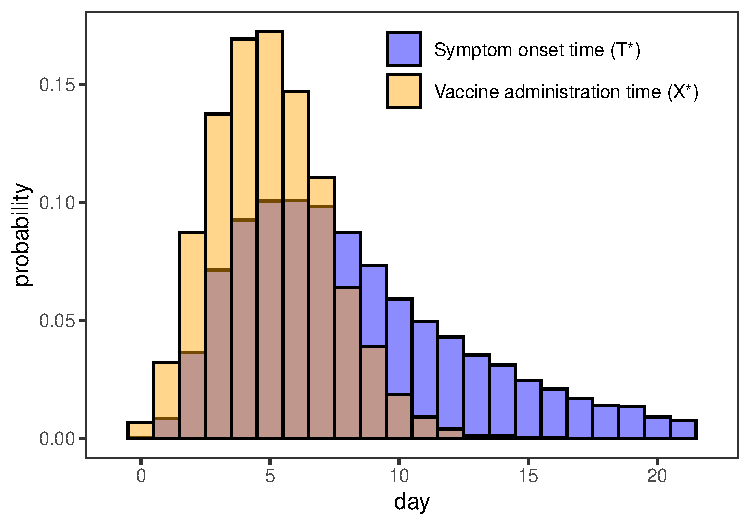
\includegraphics{../3_figures/dist.pdf}
    \caption{Distribution of simulated vaccination times ($X^*$) among vaccinated and symptom onset times ($T^*$) among cases when $VE = 0$ over the 21 days of follow up showing the degree of overlap.}
    \label{fig:example_overlap}
\end{figure}

In each simulation, we estimate vaccine efficacy using three different strategies:
\begin{enumerate}
    \item \textit{naive, leave} - a simple comparison of the ``ever vaccinated'' and ``never vaccinated'' using the relative risk regression model $\Pr[Y = 1 \mid X] = \operatorname{exp}\{\beta_0 + \beta_1 I(X < 21)\}$ and vaccine efficacy is estimated as $\widehat{VE} = 1 - \exp(\widehat{\beta_1})$.
    \item \textit{naive, move} - those who receive vaccine after developing symptoms are re-classified as ``unvaccinated'', i.e. we use the relative risk regression model $\Pr[Y = 1 \mid X] = \operatorname{exp}\{\beta_0 + \beta_1 I(X < T)\}$ where $I(X<T)$ implies only those who receive vaccine prior to symptom onset are ``vaccinated'' and vaccine efficacy is estimated as $\widehat{VE} = 1 - \exp(\widehat{\beta_1})$ as before.
    \item \textit{target trial} - we emulate a sequence of nested daily trials by taking those who are symptom free and unvaccinated prior to start and compare those are vaccinated on that day to those who are not. In each trial, we censor the unvaccinated when they become vaccinated and use inverse-probability of censoring weights to account for informative censoring. These nested trials are combined and vaccine effectiveness is estimated using standardized cumulative incidence curves from a pooled logistic regression and standard errors are estimated using cluster-robust variance estimator.
\end{enumerate}
The first two are strategies that we have seen used in observational studies of post-exposure vaccination and the last is the one proposed in this paper.

\begin{figure}[t]
  \centering
  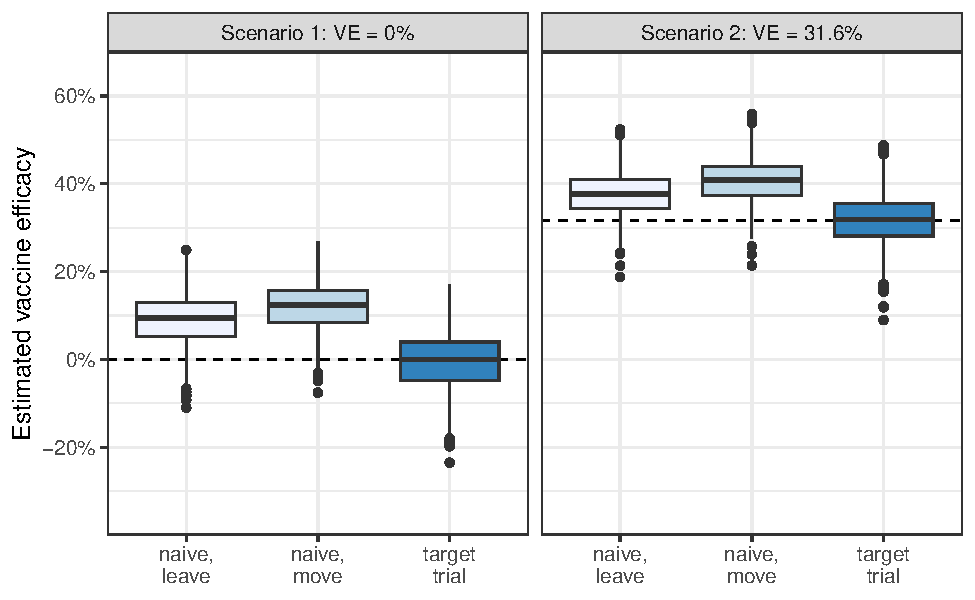
\includegraphics{../3_figures/sim_rr.pdf}
  \caption{Simulated $VE$ estimates compared to the truth for the three estimation strategies described in section \ref{sec:simulation}. Based on 1000 monte carlo simulations. Dashed line shows true value in each scenario. \label{fig:sim_results}}
\end{figure}

We drew datasets of size 1000, estimated the $VE$ under each estimation strategy, and repeated the process 1000 times to calculate the bias and efficiency. In Figure \ref{fig:sim_results} we compare estimates to the truth across the first two scenarios. Under the null, the naive approaches are upwardly biased due to immortal time bias (i.e. by definition vaccinated have to survive long enough to be vaccinated while unvaccinated are at risk at all time points), while the target trial approaches yield valid estimates. This persists in scenario 2 where $VE = 31.6\%$, although the relative bias of the first approach is somewhat offset by the fact that those vaccinated after developing symptoms are included with vaccinated. In scenario 3, where vaccine efficacy varies with postexposure timing, the naive approaches still produce biased estimates, with larger bias for greater postexposure delays. The target trial approach yields unbiased estimates of vaccine effectiveness at all time points (Figure \ref{fig:sim_hetx}). 

Another common approach to account for immortal time is to split follow up at the time of vaccination among the vaccinated and use a time-varying specification of the Cox proportional hazards model to estimate $VE$. In Figure \ref{fig:sim_hr} in the appendix, we show this approach also yields unbiased estimates of postexposure vaccine efficacy when evaluated using one minus the hazard ratio rather than cumulative incidence (the latter could, in theory at least, be obtained by combining with a suitable estimator of the baseline hazard, but this is uncommon). However, in practice, this method imposes restrictions on appropriate adjustment for time-varying confounding that is almost certainly present in most real world applications. 

Finally, we also evaluated how performance varies with the degree of overlap between vaccination and symptom onset. Specifically, we varied the mean of the log-normal distribution used to generate the symptom onset times, with larger means corresponding to later symptom onset and thus less overlap. In Figure \ref{fig:sim_overlap}, we show that the bias of the naive approaches increases as the mean onset time gets shorter while both the target trial and time-varying Cox approaches remain unbiased. This suggests that the target trial approach may be particularly useful in settings with high overlap between vaccination and symptom onset or those in which the majority of cases occur prior to vaccine being administered.

\section{Discussion} \label{sec:discussion}
Accurate assessments of postexposure efficacy of vaccines against the onset of disease could be useful for curbing the worst sequelae of many pathogens, but trials are often infeasible due to logistical, regulatory, or financial constraints. Here, we specified target trials for postexposure vaccination and describe how to emulate them using observational data. Using the example of mpox vaccines, we discussed some of the unique challenges of emulating postexposure vaccination trials, including the central role played by the distribution of vaccination times and the incubation period. Throughout we emphasize the clarifying role of the target trial framework and conclude with simulations showing how emulating the trial can help avoid several common biases in observational analyses. 

Previous studies have emulated trials of pre-exposure vaccines, particularly during the COVID-19 pandemic \cite{dagan_bnt162b2_2021,dickerman_comparative_2022,cohen-stavi_bnt162b2_2022,barda_effectiveness_2021}. These studies filled gaps in the literature by emulating trials which were not feasible to implement in practice such as head-to-head comparisons of vaccines \cite{dickerman_comparative_2022}, effectiveness against new variants \cite{cohen-stavi_bnt162b2_2022}, effectiveness of boosters \cite{barda_effectiveness_2021,magen_fourth_2022}, and effectiveness in important subgroups such as children \cite{cohen-stavi_bnt162b2_2022} and the immunocompromised. Observational emulations of post-exposure vaccines could perform a similar function.

We have mostly considered postexposure trials where the goal of vaccination is to prevent the onset of clinical disease. However, other goals such as reducing severity or transmission are also possible. To emulate trials in which the goal is to reduce severity, one could simply replace onset with an alternative outcome such as hospitalization or death in the trials outlined above. 

Beyond estimating postexposure efficacy, a secondary goal of a postexposure trial could be to determine the maximum vaccination delay before efficacy falls below a certain cost-benefit threshold. This quantity is important both for policymakers communicating with high risk groups and the broader public about what to do in the event of an exposure as well as to help practitioners determine whether vaccination is still indicated upon presentation. In section \ref{sec:maxdelay} of the Appendix, we develop a formal counterfactual framework for the maximum delay and provide additional details on how to estimate it using data from an observational emulation.

As shown in our simulation, some issues related to immortal time bias could be resolved by alternative estimation strategies, such as using a time-dependent Cox model \cite{suissa_immortal_2008}. However, emulating a specific target trial helps clarify other ambiguities, provides a standard against which we can benchmark, and helps us understand when adjustment for time-varying confounding is necessary.

\clearpage

\newpage

\printbibliography

\begin{appendix}

    \renewcommand{\thefigure}{A\arabic{figure}}
    \setcounter{figure}{0}
    
    \renewcommand{\thetable}{A\arabic{table}}
    \setcounter{table}{0}
    
    \renewcommand{\theequation}{A\arabic{equation}}
    \setcounter{equation}{0}

    \newpage

    \section{Appendix}

    \subsection{Day zero designs} \label{sec:dayzero}
    In the main text, we discussed two trial designs starting on postexposure day zero. In the first, participants are enrolled on postexposure day zero, randomized, and immediately administered either vaccine or no vaccine with the goal of estimating the $\Delta$-day vaccine efficacy in the ideal case in which there is no delay between exposure and vaccination. Under perfect adherence this trial targets the estimand
    $$VE(0) = 1 - \frac{\Pr[Y^{x = 0} = 1]}{\Pr[Y^{x > \Delta} = 1]}$$
    which is likely an upper bound on vaccine efficacy under more plausible scenarios of delay. 

    In the second design, participants are still enrolled and randomized on postexposure day zero, but they are then further randomly assigned a postexposure date to receive the vaccine.  Under perfect adherence, the casual contrast of interest is now the $t$-specific vaccine efficacy
    $$VE(t) = 1 - \frac{\Pr[Y^{x = t} = 1]}{\Pr[Y^{x > \Delta} = 1]}.$$
    which could be used, for instance, to determine the time window public health officials and policymakers should advise individuals at risk of exposure to seek vaccination within if they are exposed (see Section \ref{sec:maxdelay}).

    \subsection{Fixed enrollment period designs} \label{sec:enrollment}

    Also mentioned in the main text, when the timing of vaccination is not under the strict control of the investigator, a possible design is to specify a fixed time window in which participants are eligible to be vaccinated and randomize them on the postexposure day they present. Under perfect adherence, this design could then target the $t$-specific vaccine efficacy among those presenting symptom-free, i.e.
    $$
    VE_{T > t}(t) = 1 - \frac{\Pr[Y^{x = t} = 1 \mid X \geq t, T > t]}{\Pr[Y^{x > \Delta} = 1 \mid X \geq t, T > t]} \\
    $$
    by comparing vaccine and no vaccine groups within enrollment  strata. Note that, in general, the $t$-specific vaccine efficacies, $VE_{T > t}(t)$, targeted in this trial will not be the same as the $VE(t)$ defined previously as they are conditional on presentation time and being symptom-free at enrollment. More often, in practice, the $t$-specific estimates $VE_{T > t}(t)$ are pooled together into a weighted average efficacy over the enrollment period. However, we stress caution in interpreting pooled estimates. Because participants are allowed to present naturally rather than being assigned a time at day zero, those that present earlier may be systematically different than those presenting later with respect to their risk of developing clinical disease. Therefore the pooled estimates are among a subpopulation who survive symptom-free and may not generalize to other populations with different propensities for delay. 

    \subsection{Grace period designs} \label{sec:graceperiod}

    An alternative design which also allows for delays in vaccination is to specify a \textit{grace period}, i.e. a fixed time window after randomization in which vaccination can be initiated. For example, in a postexposure trial of a varicella vaccine, the investigators stipulated that sibling contacts of varicella case were ``were identified by their primary pediatrician and referred to our department \textit{within 72 hours} of the appearance of the first skin lesion'' in the index case. Under this design, the causal target would be the average vaccine effectiveness during the $\delta$ days of the grace period, i.e.
    $$
    \overline{VE}_\delta = 1 - \frac{\Pr[Y^{g(X,\delta)} = 1]}{\Pr[Y^{x > \Delta} = 1]}
    $$ 
    where
    \begin{gather*}
        g(X,\delta): \text{get vaccinated within $\delta$ days of exposure under the expected vaccine } \\ \text{ administration pattern }  f^*(X \mid \overline{L}_t, X > t, T > t)
    \end{gather*}
    where, for instance, in the varicella trial $\delta = 3$. Although in theory randomization could occur on any postexposure day followed by $\delta$-day grace period, in practice grace periods starting from randomization on day zero are probably the most relevant. When effectiveness varies by the time since exposure, as it most certainly does for most postexposure vaccines, a design with as grace design estimates the average effectiveness \textit{under the ``natural'' time course of vaccination}, $f^*(X \mid \overline{L}_t, X > t, T > t) = f(X \mid \overline{L}_t, X > t, T > t)$. This implies that two trials identical in all respects except for the distribution of vaccinations over the grace period could yield substantially different estimates. Therefore, a trialist pursuing this design has to strike a balance when defining a grace period between ensuring the period is short enough that benefit is immunologically possible and the trial is adequately powered, but also long enough that the regime is clinically feasible under reasonable assumptions about how quickly patients are notified of their exposure to a case and can access a vaccine in the real world. Properly conceived a grace period design can provide evidence about average effectiveness of postexposure vaccination administered within a certain window under real world conditions. As such it may be a more useful estimate for population planning or modeling studies than those produced by the stratified design above. When there's no effect modification by initiation or onset time, the average effectiveness is equal to $VE(t)$ standardized over the distribution of vaccine administration times during the grace period, i.e.
    $$\overline{VE}_\delta = \sum_{t = 1}^\delta VE(t) \times f^*_X(t \mid \overline{L}_t, X > t, T > t).$$

    \subsection{Additional emulation details}
    Here, we demonstrate the data manipulation steps to emulate the three trial designs ---day zero, fixed enrollment period, and grace period--- discussed above using observational data. These steps are pre-requisites for emulating the analysis that would have been conducted in the ideal trial, but will not, by themselves, ensure the effect estimated from the observational data is equivalent to the one that would be observed in the trial (accounting for sampling variablility). As in all observational research, additional untestable assumptions, notably exchangeability, consistency, and positivity, will be required. 

    Two crucial differences between a randomized trial and an observational study are that 1) the former has a well defined start of follow up, or \textit{time zero}, from which study outcomes are assessed and 2) all participants are assigned a particular treatment strategy. By contrast observational studies generally do not have a uniquely defined time zero and participants may have data consistent with multiple treatment strategies. Therefore, when emulating a trial certain data manipulations are often applied to the observational data to solve these issues. 

    When emulating a fixed enrollment period design, the problem is that participants in the observational data often meet the eligibility criteria at multiple time points, that is there is no uniquely defined time zero from which to start follow up. For instance, consider a postexposure vaccination trial in which participants are eligible anytime in the first 5 days after exposure if they have no previous vaccination history and no symptoms at presentation. In a real trial the participant would be enrolled and randomized on a particular day and that will be their time zero. In the observational data, a participant may meet these criteria continuously, for instance between days 0 and 4. The question is then when should their follow-up start? On day 0, 1, 2, 3, or 4? The choice has to be applied equivalently to vaccinated and unvaccinated participants to avoid \textit{immortal time bias}. One possibility is to randomly choose a start time among the days they are eligible. However, a more efficient choice is to use every eligible time by emulating a sequence of multiple nested target trials each with a different start. A natural choice for postexposure vaccination for a pathogen with a relatively short incubation period is to emulate a series of daily nested trials, i.e. on day zero condition on those who meet the eligibility criteria and compare those who are vaccinated on that day to those who are unvaccinated on that day, and then repeat on all days within the fixed enrollment period (schematic Figure \ref{fig:design1}). Participants in the observational study can be enrolled in trials starting on multiple days as long as they meet the eligibility criteria.
    
    To demonstrate the required data manipulation steps, consider the six individuals shown in Table \ref{tab:example1} with vaccination and symptom onset times recorded during a hypothetical observational study. To emulate a trial with a fixed five day enrollment period postexposure, we create one copy of the dataset for each trial day. Then in each copy we apply the proper eligibility criteria (e.g. individuals should be disease-free and not vaccinated on a previous day) and assign those vaccinated on that trial day to be ``vaccinated'' and those who have not been vaccinated yet to be ``unvaccinated''. For example, individual 2 in Table \ref{tab:example1} is vaccinated on on day 2 and doesn't develop symptoms, therefore in the emulation they will participate in 3 trials (i.e. those starting on postexposure day 0, 1, and 2). In trials starting after postexposure day 2 they are no longer eligible because they have already been vaccinated. In each trial, follow up time is adjusted to start on the postexposure day of interest and end either at symptom onsent or at the maximum follow up day which may be fixed from the index exposure day or be of fixed length from the trial day. In per protocol analyses, individuals in each nested trial are censored when they deviate from their baseline assignment in that trial. For example, individual 3 in Table \ref{tab:example1} is unvaccinated in trials starting on days 0 through 3, but in each of these trials is censored on day 4 in the per protocol analysis because they deviate from their baseline assignment by becoming vaccinated.
    
    \begin{table}[t]
        \small
        \centering
        \caption{Enrollment of six hypothetical individuals in daily nested trials for 5-day vaccination window based on observed data.\label{tab:example1}}
        \begin{tabular}{cC{0.9in}C{0.9in}C{1in}C{1in}C{0.9in}C{0.9in}}
        \toprule
        \makecell[c]{ID} & \makecell[c]{Vaccination \\ (1: yes, 0: no)} & \makecell[c]{Day of \\ vaccination} & \makecell[c]{Clinical disease \\ (1: yes, 0: no)} & \makecell[c]{Day of \\ disease onset} & \makecell[c]{No. of trials \\ enrolled} \\
        \midrule
            1 & 1 & 0 & 0 & - & 1 (0) \\
            2 & 1 & 2 & 0 & - & 3 (0-2) \\
            3 & 1 & 4 & 1 & 8 & 5 (0-4) \\
            4 & 1 & 7 & 1 & 3 & 4 (0-3) \\
            5 & 0 & - & 0 & - & 6 (0-5) \\
            6 & 0 & - & 1 & 5 & 6 (0-5) \\
        \bottomrule
        \end{tabular}
    \end{table}

    Once we have completed the necesary data manipulation steps to emulate the nested sequence of trials, analysis of both the intent-to-treat and per-protocol effects of postexposure vaccination can be conducted as described in the main text. One approach would be to estimate the $t$-specific $VE_{T > t}(t)$ separately in each nested trial. However, this assumes we observe sufficient numbers of individuals receiving a vaccine on each day to obtain reliable estimates. In practice, we can increase efficiency by pooling across trials and fitting a model such as
    \begin{equation}\Pr[D_{t+1} = 1 \mid D_t = 0, X, Z, L_t] =  \operatorname{expit}\{\psi_0 \lambda(X + t) + \psi_1 Z f(X) + \psi_2 L_t\}
    \end{equation}\label{eqn:fixed}
    where $\lambda(X + t)$ is the unvaccinated odds of symptom onset,  $Z$ is an indicator of baseline ``assignment'' in the trial, $X$ is the postexposure day that the trial starts, $L_t$ is a vector of baseline covariates sufficient to ensure exchangeability at baseline, $t$ is follow up time counting from $X$, and $f(X)$ is a function of vaccination day. We can allow $f(X)$ and $\lambda(X + t)$ to be a member of a class of flexible such as restricted cubic splines. The $\widehat{VE}_{T > t}(t)$ curve can be estimated either from the hazard ratios or from standardized cumulative incidence curves depending on effect measure of interest. To estimate per protocol effects we censor participants when their data deviates from their ``assigned'' regime and then adjust for possible time-varying selection bias using any g-method such as inverse-probability of censoring weights. Additionally, because we are using the same participant in multiple nested trials our observations are no longer independent. Therefore appropriate adjustment to our standard errors is necessary to account for possible correlation across observations. Adjustment can be made either by using a cluster-robust variance estimator or the bootstrap. 

    When emulating a day zero trial in which participants are randomized to a particular delay, the problem is instead that participants in the observational data will have data consistent with multiple treatment regimes. Consider a trial where participants are randomized on day zero to one of the following strategies: (1) receive vaccine on day zero, (2) receive vaccine on day one, (3) receive vaccine on day two, (4) receive vaccine on day three, or (5) to receive no vaccine over the follow up period (schematic Figure \ref{fig:design2}). In a real trial participants would be assigned to one of the five regimes at the start. In the observational data, however, some individuals will get vaccinated on day 0 and therefore only have data compatible with the first strategy, but others will not get vaccinated on day zero and will have data compatible with multiple strategies at baseline. The question is now which strategy should we assign them to? As in the sequential design, one option is to pick a single strategy at random from the strategies their data is consistent with. However, again the more efficient choice is to assign them to all possible strategies by creating exact copies ---often called clones--- of each of these individuals in the dataset and assign each clone to a different strategy. 

    To demonstrate the required data manipulation steps, let's return to the six hypothetical individuals from Table \ref{tab:example1}, but now in Table \ref{tab:example2} we will use their data to emulate a day zero trial in which participants are randomized to strategies (1)-(5) in previous paragraph. Starting with the first individual, they are vaccinated on day zero and therefore have data consistent only with strategy (1), thus they are not cloned. The second individual, however, is not vaccinated until day 2 and therefore at time zero they have data consistent with any of the strategies (1)-(5), thus we make five clones of the second individual by copying their data five times and assigning each observation to a different regime. We then follow each clone forward and censor them when they deviate from their assigned regime. For instance, we know the second individual is vaccinated on day 2, therefore on day 2 we censor all clones except the one assigned to strategy (3). Importantly, if the individual has symptoms before any clone is censored, as is the case for individual 4, then all clones will have symptoms and therefore the case is assigned to all strategies strategies. This multiple allocation of events prevents the bias that could arise if events occurring during the delay period are systematically assigned to one of the five strategies only.

    \begin{table}[t]
        \small
        \centering
        \caption{Emulation of day zero trial with five vaccination delay strategies using data from six hypothetical individuals.\label{tab:example2}}
        \begin{tabular}{cC{0.9in}C{0.9in}C{1in}C{1in}C{0.9in}}
        \toprule
        \makecell[c]{ID} & \makecell[c]{Vaccination \\ (1: yes, 0: no)} & \makecell[c]{Day of \\ vaccination} & \makecell[c]{Clinical disease \\ (1: yes, 0: no)} & \makecell[c]{Day of \\ disease onset} & \makecell[c]{No. of regimes \\ followed} \\
        \midrule
            1 & 1 & 0 & 0 & - & 1 (1) \\
            2 & 1 & 2 & 0 & - & 5 (1-5) \\
            3 & 1 & 4 & 1 & 8 & 5 (1-5) \\
            4 & 1 & 7 & 1 & 3 & 5 (1-5) \\
            5 & 0 & - & 0 & - & 5 (1-5) \\
            6 & 0 & - & 1 & 5 & 5 (1-5) \\
        \bottomrule
        \end{tabular}
    \end{table}

    To analyze the data from the emulated day zero trial, we could estimate the $VE(t)$ separately by comparing each delay strategy, e.g. (1)-(4), to the ``never vaccinate'' strategy (5). Once again, however, we could increase efficiency by pooling across trials and fitting a model such as
    \begin{equation}
        \Pr[D_{t+1} = 1 \mid D_t = 0, Z, L_t] =  \operatorname{expit}\{\psi_0 \lambda(t) + \psi_1f(Z) + \psi_2 L_t\}
    \end{equation} \label{eqn:dayzero}
    where $Z$ is now a discrete variable with levels for each delay regime (with 0 being the ``never vaccinate'' strategy) and other variables are defined as previously. As previously, the $\widehat{VE}(t)$ curve can be estimated either from the hazard ratios or from standardized cumulative incidence curves depending on effect measure of interest. Adjustment for the nonindepence of the cloned observations can be made either by using a cluster-robust variance estimator or the bootstrap. 

    Finally, when emulating the grace period design the challenges are similar to those in the day zero trial in which participants are randomized to a delay strategy, i.e. some participants in the observational study have data consistent with multiple regimes. Consider a trial where participants are randomized at day zero to either (1) receive vaccine sometime within the first five days postexposure or (2) to receive no vaccine over the follow up period (schematic Figure \ref{fig:design3}). Once again, if the trial were actually conducted everyone would have an unambiguous assignment at time zero. However, in the observational data individuals who receive vaccine after day zero have data consistent with both strategies in the period before receiving the vaccine. This is important when considering some individuals may acquire symptoms prior to receiving vaccination during the grace period, in which case to which strategy should they be assigned? The solution, as before, is to create clones when individuals have data consistent with multiple regimes, assign each clone to a regime, and then censor them if they deviate from their assigned regime. 

    To demonstrate the required data manipulation steps, we return again to the same six hypothetical individuals, but now in Table \ref{tab:example3} we will use their data to emulate a trial with a five day grace period. Starting with the first individual, they are vaccinated on day zero and therefore have data consistent only with strategy (1) and therefore they are not cloned. The second individual, however, is not vaccinated until day 2 and therefore at time zero has data consistent both strategies (1) and (2), thus we make two clones of the second individual by copying their data and assigning each observation to one of the two regimes. We then follow each clone forward and censor them when they deviate from their assigned regime. For instance, we know the second individual is vaccinated on day 2, therefore on day 2 we censor the clone assigned to regime (2), i.e. receive no vaccine over the follow up period. Again, if the individual has symptoms before any clone is censored, as is the case for individual 4, then all clones will have symptoms and therefore the case is assigned to all strategies strategies. This double allocation of events prevents the bias that could arise if events occurring during the grace period are systematically assigned to one of the two strategies only. 

    \begin{table}[t]
        \small
        \centering
        \caption{Emulation of trial with five day grace period vaccination using data from six hypothetical individuals.\label{tab:example3}}
        \begin{tabular}{cC{0.9in}C{0.9in}C{1in}C{1in}C{0.9in}}
        \toprule
        \makecell[c]{ID} & \makecell[c]{Vaccination \\ (1: yes, 0: no)} & \makecell[c]{Day of \\ vaccination} & \makecell[c]{Clinical disease \\ (1: yes, 0: no)} & \makecell[c]{Day of \\ disease onset} & \makecell[c]{No. of regimes \\ followed} \\
        \midrule
            1 & 1 & 0 & 0 & - & 1 (1) \\
            2 & 1 & 2 & 0 & - & 2 (1-2) \\
            3 & 1 & 4 & 1 & 8 & 2 (1-2) \\
            4 & 1 & 7 & 1 & 3 & 2 (1-2) \\
            5 & 0 & - & 0 & - & 2 (1-2) \\
            6 & 0 & - & 1 & 5 & 2 (1-2) \\
        \bottomrule
        \end{tabular}
        \end{table}

    To analyze the emulated grace period design, we can estimate the average vaccine effectiveness over the grace period $\overline{VE}_\delta$ by fitting the model 
    $$\Pr[D_{t+1} = 1 \mid D_t = 0, Z, L_t] =  \operatorname{expit}\{\psi_0 \lambda(t) + \psi_1 Z + \psi_2 L_t\}$$
    where $Z$ is an indicator of the vaccination strategy and the other variables are defined as previously. As previously, the $\overline{VE}_\delta$ curve can be estimated either from the hazard ratios or from standardized cumulative incidence curves depending on effect measure of interest. When analyzing designs with grace periods, the intention-to-treat effect cannot be estimated because almost everyone will contribute a clone to each of the treatment strategies. Because each individual is assigned to all strategies at baseline, a contrast based on baseline assignment (i.e., an ``intention-to-treat analysis'') will compare groups with essentially identical outcomes. Therefore, analyses with grace period at baseline are geared towards estimating some form of per-protocol effect. To estimate per protocol effects, we again censor participants when their data deviates from their ``assigned'' regime and then adjust for possible time-varying selection bias using any g-method such as inverse-probability of censoring weights. Note that, to emulate a well-defined vaccination strategy the expected rate of vaccination over the grace period $f^*(X \mid \overline{L}_t, X > t, T > t)$ should be specified and then the per-protocol effect under this vaccination strategy can be emulated by multiplying the inverse probability weights by a suitable factor. Finally, as with the day zero design adjustment for the nonindepence of the cloned observations can be made either by using a cluster-robust variance estimator or the bootstrap. 

    

    

    \newpage 
    \clearpage
    \begin{figure}[p]
    \centering
    \begin{tikzpicture}[> = stealth, shorten > = 1pt, auto, node distance = 1.5cm, thick]
    
    \node[circle,draw=none] (y0) {$Y$};
    \node[circle,draw=none] (y1) [below of=y0] {$Y$};
    \node[circle,draw=none] (y2) [below of=y1] {$Y$};
    \node[circle,draw=none] (y3) [below of=y2] {$Y$};
    \node[circle,draw=none] (d) [below of=y3] {\large $\vdots$};
    \node[circle,draw=none] (y4) [below of=d] {$Y$};
    \node[circle,draw=none] (y5) [below of=y4] {$Y$};

    \node[circle,draw,minimum size =1cm] (a03) [left of=y0] {$1$};
    \node[circle,draw,minimum size =1cm] (a02) [left of=a03] {$1$};
    \node[circle,draw,minimum size =1cm] (a01) [left of=a02] {$1$};
    \node[circle,draw,minimum size =1cm] (a0)  [left of=a01] {$1$};

    \node[circle,draw,minimum size =1cm] (a13) [left of=y1] {$0$};
    \node[circle,draw,minimum size =1cm] (a12) [left of=a13] {$0$};
    \node[circle,draw,minimum size =1cm] (a11) [left of=a12] {$0$};
    \node[circle,draw,minimum size =1cm] (a1)  [left of=a11] {$0$};

    \node[regular polygon,regular polygon sides=4, draw,fill=gray!30,minimum size =1.25cm] (l0) [below left=0.01cm and 1.5cm of a0] {$ $};  
    
    \node[circle,draw=none] (day0) [left= 1cm of l0] {Trial $0$};

    \path[->] (l0) edge node {} (a0);
    \path[->] (l0) edge node {} (a1);
    \path[->] (a0) edge node {} (a01);
    \path[->] (a1) edge node {} (a11);

    \path[->] (a11) edge node {} (a12);
    \path[->] (a12) edge node {} (a13);
    \path[->] (a13) edge node {} (y1);

    \path[->] (a01) edge node {} (a02);
    \path[->] (a02) edge node {} (a03);
    \path[->] (a03) edge node {} (y0);

    \node[circle,draw,minimum size =1cm] (a23) [left of=y2] {$1$};
    \node[circle,draw,minimum size =1cm] (a22) [left of=a23] {$1$};
    \node[circle,draw,minimum size =1cm] (a21) [left of=a22] {$1$};

    \node[circle,draw,minimum size =1cm] (a33) [left of=y3] {$0$};
    \node[circle,draw,minimum size =1cm] (a32) [left of=a33] {$0$};
    \node[circle,draw,minimum size =1cm] (a31) [left of=a32] {$0$};

    \node[regular polygon,regular polygon sides=4, draw,fill=gray!30,minimum size =1.25cm] (l11) [below left=0.01cm and 1.5cm of a21] {$ $};  
    \node[regular polygon,regular polygon sides=4, draw,fill=gray!30,minimum size =1.25cm] (l10) [left of=l11] {$ $};  

    \node[circle,draw=none] (day1) [left= 1cm of l10] {Trial $1$};

    \path[->] (l11) edge node {} (a21);
    \path[->] (l11) edge node {} (a31);

    \path[->] (a21) edge node {} (a22);
    \path[->] (a22) edge node {} (a23);
    \path[->] (a23) edge node {} (y2);

    \path[->] (a31) edge node {} (a32);
    \path[->] (a32) edge node {} (a33);
    \path[->] (a33) edge node {} (y3);

    \node[circle,draw=none] (dd) [below of=a32] {\large $\ddots$};

    \node[circle,draw=none] (dv) [left=4.1cm of dd] {\large $\vdots$};

    \node[circle,draw,minimum size =1cm] (a43) [left of=y4] {$1$};

    \node[circle,draw,minimum size =1cm] (a53) [left of=y5] {$0$};

    \node[regular polygon,regular polygon sides=4, draw,fill=gray!30,minimum size =1.25cm] (l33) [below left=0.01cm and 1.5cm of a43] {$ $};  
    \node[regular polygon,regular polygon sides=4, draw,fill=gray!30,minimum size =1.25cm] (l32) [left of=l33] {$ $};  
    \node[regular polygon,regular polygon sides=4, draw,fill=gray!30,minimum size =1.25cm] (l31) [left of=l32] {$ $};  
    \node[regular polygon,regular polygon sides=4, draw,fill=gray!30,minimum size =1.25cm] (l30) [left of=l31] {$ $};  

    \node[circle,draw=none] (dayd) [left= 1cm of l30] { Trial $\delta$};

    \path[->] (l33) edge node {} (a43);
    \path[->] (l33) edge node {} (a53);

    \path[->] (a43) edge node {} (y4);
    \path[->] (a53) edge node {} (y5);

    \end{tikzpicture}
   
    \caption{Schematic of nested daily trial design, on each day participants are assigned to vaccine or no vaccine, possibly conditional on their history up to that day.}
    \label{fig:design1}
    \end{figure}

    \clearpage
    \begin{figure}[p]
        \centering
        \begin{tikzpicture}[> = stealth, shorten > = 1pt, auto, node distance = 1.5cm, thick]

            \node[circle,draw=none] (y0) {$Y$};
            \node[circle,draw=none] (y1) [below of=y0] {$Y$};
            \node[circle,draw=none] (y2) [below of=y1] {$Y$};
            \node[circle,draw=none] (y3) [below of=y2] {$Y$};
            \node[circle,draw=none] (y4) [below of=y3] {$Y$};
        
            \node[circle,draw,minimum size =1cm] (a03) [left of=y0] {$1$};
            \node[circle,draw,minimum size =1cm] (a02) [left of=a03] {$1$};
            \node[circle,draw,minimum size =1cm] (a01) [left of=a02] {$1$};
            \node[circle,draw,minimum size =1cm] (a0)  [left of=a01] {$1$};
        
            \node[circle,draw,minimum size =1cm] (a13) [left of=y1] {$1$};
            \node[circle,draw,minimum size =1cm] (a12) [left of=a13] {$1$};
            \node[circle,draw,minimum size =1cm] (a11) [left of=a12] {$1$};
            \node[circle,draw,minimum size =1cm] (a1)  [left of=a11] {$0$};
            
        
            \path[->] (a0) edge node {} (a01);
            \path[->] (a1) edge node {} (a11);
        
            \path[->] (a11) edge node {} (a12);
            \path[->] (a12) edge node {} (a13);
            \path[->] (a13) edge node {} (y1);
        
            \path[->] (a01) edge node {} (a02);
            \path[->] (a02) edge node {} (a03);
            \path[->] (a03) edge node {} (y0);
        
            \node[circle,draw,minimum size =1cm] (a23) [left of=y2] {$1$};
            \node[circle,draw,minimum size =1cm] (a22) [left of=a23] {$1$};
            \node[circle,draw,minimum size =1cm] (a21) [left of=a22] {$0$};
            \node[circle, draw, minimum size =1cm] (a20) [left of=a21] {$0$}; 
    
            \node[circle,draw,minimum size =1cm] (a33) [left of=y3] {$1$};
            \node[circle,draw,minimum size =1cm] (a32) [left of=a33] {$0$};
            \node[circle,draw,minimum size =1cm] (a31) [left of=a32] {$0$};
            \node[circle, draw, minimum size =1cm] (a30) [left of=a31] {$0$};  
     
            \node[regular polygon,regular polygon sides=4, draw,fill=gray!30,minimum size =1.25cm] (l0) [left=1.5cm of a20] {$ $};  
    
            \path[->] (l0) edge node {} (a0);
            \path[->] (l0) edge node {} (a1);
            \path[->] (l0) edge node {} (a20);
            \path[->] (l0) edge node {} (a30);
    
            \path[->] (a20) edge node {} (a21);
            \path[->] (a21) edge node {} (a22);
            \path[->] (a22) edge node {} (a23);
            \path[->] (a23) edge node {} (y2);
    
            \path[->] (a30) edge node {} (a31);
            \path[->] (a31) edge node {} (a32);
            \path[->] (a32) edge node {} (a33);
            \path[->] (a33) edge node {} (y3);
        
            \node[circle,draw,minimum size =1cm] (a43) [left of=y4] {$0$};
            \node[circle, draw, minimum size =1cm] (a42) [left of=a43] {$0$};  
            \node[circle, draw, minimum size =1cm] (a41) [left of=a42] {$0$};  
            \node[circle, draw, minimum size =1cm] (a40) [left of=a41] {$0$};  
    
        
            \path[->] (l0) edge node {} (a40);
        
            \path[->] (a40) edge node {} (a41);
            \path[->] (a41) edge node {} (a42);
            \path[->] (a42) edge node {} (a43);
            \path[->] (a43) edge node {} (y4);
    
            \end{tikzpicture}
            \caption{Schematic of trials in which participants are randomized on day zero to a specific vaccination delay strategy.}
            \label{fig:design2}
    \end{figure}

    \begin{figure}[p]
        \centering
        \begin{tikzpicture}[> = stealth, shorten > = 1pt, auto, node distance = 1.5cm, thick]

            % \node[circle,draw=none] (y0) {$Y$};
            % \node[circle,draw=none] (y1) [below of=y0] {$Y$};
            % \node[circle,draw=none] (y2) [below of=y1] {$Y$};
            % \node[circle,draw=none] (y3) [below of=y2] {$Y$};
            % \node[circle,draw=none] (d) [below of=y3] {\large $\vdots$};
            \node[circle,draw=none] (y4) {$Y$};
            \node[circle,draw=none] (y5) [below of=y4] {$Y$};
        
            \node[circle,draw,minimum size =1cm] (a43) [left of=y4] {$1$};
            \node[circle, draw, dashed, minimum size =1cm] (a42) [left of=a43] {$?$};  
            \node[circle, draw, dashed, minimum size =1cm] (a41) [left of=a42] {$?$};  
            \node[circle, draw, dashed, minimum size =1cm] (a40) [left of=a41] {$?$};  
    
            \draw [decorate,decoration={brace,amplitude=10pt, raise =1cm}]
            (a40.center) -- (a42.center) node [yshift=1.5cm,midway] 
            {$\delta$-day grace period};

            \node[circle,draw,minimum size =1cm] (a53) [left of=y5] {$0$};
            \node[circle, draw, minimum size =1cm] (a52) [left of=a53] {$0$};  
            \node[circle, draw, minimum size =1cm] (a51) [left of=a52] {$0$};  
            \node[circle, draw, minimum size =1cm] (a50) [left of=a51] {$0$};  
    
            \node[regular polygon,regular polygon sides=4, draw,fill=gray!30,minimum size =1.25cm] (l30) [below left=0.01cm and 1.5cm of a40] {$ $};  
        
            \path[->] (l30) edge node {} (a40);
            \path[->] (l30) edge node {} (a50);
        
            \path[->] (a40) edge node {} (a41);
            \path[->] (a50) edge node {} (a51);
            \path[->] (a41) edge node {} (a42);
            \path[->] (a51) edge node {} (a52);
            \path[->] (a42) edge node {} (a43);
            \path[->] (a52) edge node {} (a53);
            \path[->] (a43) edge node {} (y4);
            \path[->] (a53) edge node {} (y5);
    
            \end{tikzpicture}
            \caption{Schematic of trials with a grace period, participants are randomized to a strategy starting on day zero and given a fixed length time window in which they can initiate and then sustain thereafter.}
            \label{fig:design3}
    \end{figure}

    \clearpage

    \subsection{Adjusting trial outcomes based on biology}
    Sometimes there is strong biological theory or evidence about the postexposure window in which vaccination is likely to be most successful, for instance, when data from postvaccination serological assessments of antibody responses suggests meaningful change in immune responses occurs only after 7 days. In this case, there may be interest in restricting the time frame in which events count against vaccination. In a trial, this may be handled by re-defining the outcome such that only cases which occur after 7 days are counted as events. Cases that occur prior to this are not counted in either trial arm. This is how outcomes were defined, for instance, in many of the trials of SARS-CoV-2 vaccines. 
        
    In observational emulations, we can similarly re-define vaccination outcomes based on biology, however we have to be careful to ensure that the new definitions are applied fairly across vaccination groups. In traditional analyses, bias can occur when all unvaccinated cases are counted from day zero but vaccinated cases are counted from the day of vaccination. This is fixed when using either the sequential daily trials or the clone-censor-weighting approaches described previously because time zero is properly aligned in both groups.

    \subsection{Measures of vaccine efficacy}
    In the main text, we defined vaccine efficacy in terms of the cumulative incidence of symptoms or disease over the follow up period, e.g.
    $$
    VE(t) = 1 - \frac{\Pr[Y^{x=t} = 1]}{\Pr[Y^{x > \Delta} = 1]}
    $$ 
    comparing vaccination regimes vaccinated on day $t$ and never vaccinated over follow up. However, it is also common in the literature to see vaccine efficacy defined instead in terms of hazards, e.g.
    $$
    VE_\lambda(t) = 1 - \frac{\lambda^{x=t}(t)}{\lambda^{x > \Delta}(t)}
    $$ 
    where $\lambda(t)$ is the (average) hazard rate over the follow up period. In the applied literature, these are sometimes used interchangeably even though they will rarely coincide, e.g. they will not coincide when hazard rates are nonconstant or heterogeneous or nonproportional. In the causal literature, there is a preference against causal hazard ratios particularly when they are time-varying (as they almost certainly are in practice) as they condition on survival and therefore introduce possible selection bias by construction. 

    However, in their seminal work, Smith et al showed that patterns in $VE(t)$ and $VE_\lambda(t)$ could, in some circumstances, help elucidate the mechanism of action of a particular vaccine, for instance to help distinguish whether a vaccine produces ``all-or-none'' or ``leaky'' protection against infection. 

    \subsection{Determining maximum postexposure vaccination delay} \label{sec:maxdelay}
    When setting guidelines for postexposure vaccination, a common problem is determining the maximum vaccination delay before efficacy falls below a certain cost-benefit threshold. This quantity is important both for policymakers communicating with high risk groups and the broader public about what to do in the event of an exposure as well as to help practitioners determine whether vaccination is still indicated upon presentation. Absent clear biology or immune response data, it can be difficult to determine empirically even when postexposure trials are possible as trial participants are generally only assigned to vaccine or no vaccine/placebo not to a specific day to be vaccinated. In this section, we suggest a methods for estimating the maximum delay based on a pre-specified minimum efficacy bound. In principle, these methods could be applied either in a randomized trial where the day of vaccination is not strictly controlled or in an observational emulation. 
 
    Suppose $u(Y^x, t)$ is a utility function quantifying the health benefits of vaccination on postexposure day $x$ of a person who is symptom-free at time $t$. If $V$ is a subset or possibly all of baseline covariates $L_0$ defining a subpopulation of interest, such as certain high risk exposure groups, then the conditional mean
    $$m(x, t, v) \equiv E[u(Y^x, t) \mid V = v]$$
    is the expected utility under a hypothetical policy in which everyone in the subpopulation receives vaccination prior to $x$ viewed from the perspective of time $t$. Comparing the expected utility $m(x, t, v)$ for different values of $x$ quantifes the casual effect of interest. To determine the optimal guidance regarding postexposure delays, we want to find the maximum value of $x$ in which 
    utility in the subpopulation of interest remains above some minimum viable threshold viewed from $t$, i.e.
    $$x_{opt}(v, t) \equiv \operatorname{argmax}_{x \in \mathcal{X}} \{m(x, t, v) \geq \theta_{min} \}$$
    
    A simple example of $m(x, t, v)$ is the vaccine efficacy if everyone were vaccinated on day $x$ among those with $T > t$ in the full population, i.e. $VE(x^*, t)$, where
    $$VE(x^*, t) \equiv 1 - \frac{\Pr[Y^{x=x^*} = 1 \mid T > t]}{\Pr[Y^{x > \Delta} = 1 \mid T > t]}$$
    in which case we want to solve  
    $$x_{opt}(t) = \operatorname{argmax}_{x^* \in \mathcal{X}} \{VE(x^*, t) \geq \theta_{min} \}$$
    Two interesting values of $t$ to consider are:
    \begin{enumerate}
        \item $VE(x^*, 0)$, that is the effectiveness after a delay of $x^*$ days viewed from the perspective of everyone still at risk at time 0. 
        \item $VE(x^*, x^*)$, that is the effectiveness of getting vaccinated today among those symptom-free at time $t = x^*$.
    \end{enumerate}
    Each answers a slightly different question and may be relevant under different circumstances. The second is more relevant for practitioners counseling patients who present symptom-free on their options after exposure, while the first is more relevant for public health guidance telling those currently unexposed how quickly they need to get to a clinic after exposure. 

    To determine the maximum delay conditional on survival, one approach would be to use the stratified estimates $\widehat{VE}_{T > t}(t)$ from each of the nested daily trial emulations as $VE_{T > t}(t) = VE(x^*, x^*)$ for $t = x^*$ and then determine the maximum value of $t$ where  $\widehat{VE}_{T > t}(t)$ remains above the threshold. However, this assumes we observe sufficient numbers of individuals being vaccinated on each day to obtain reliable estimates. In practice, we might prefer to increase efficiency by pooling across trials and fitting a model such as that in \ref{eqn:fixed}. We can then estimate the $\widehat{VE}_{T > t}(t)$ curve either from estimated hazard ratios or from standardized cumulative incidence curves depending on effect measure of interest and using inverse probability of censoring weights to adjust for nonadherence among unvaccinated where applicable.

    To determine the maximum day zero delay, again one approach would be to calculate $\widehat{VE}(t)$ separately by comparing each delay strategy to the ``never vaccinate'' strategy from the day zero trial emulation with multiple strategies as $VE(t) = VE(x^*, 0)$ and then determine the maximum value of $t$ where  $\widehat{VE}(t)$ remains above the threshold. However,  we can also increase efficiency by pooling across trials and fitting a model such as that in \ref{eqn:dayzero}. Again, we can then estimate the $\widehat{VE}(t)$ curve either from estimated hazard ratios or from standardized cumulative incidence curves depending on effect measure of interest and using inverse probability of censoring weights to adjust for nonadherence among unvaccinated where applicable.
    
    % $$VE^x(t) = 1 - \frac{\sum_{t=0}^\Delta \Pr[D^{x}_{t+1} = 1 \mid \overline{D}^x_t = 0] \prod_{j=0}^t\Pr[D^{x}_{j+1} = 0 \mid \overline{D}^x_j = 0]}{\sum_{t=0}^\Delta \Pr[D^{\infty}_{t+1} = 1 \mid \overline{D}^\infty_t = 0] \prod_{j=0}^t\Pr[D^{\infty}_{j+1} = 0 \mid \overline{D}^\infty_j = 0]}$$

    

    % \subsection{Heterogeneity in vaccine effectiveness  }
    
    \subsection{Additional simulation details}
    
    As discussed in main text, we simulated postexposure vaccination times by drawing $X^*$ from a Poisson distribution with a mean of 5 days and then drawing an ``assignment'' indicator $Z$ from a Bernoulli distribution with probability 0.5. This mimics a trial in which vaccination timing is not controlled by investigators, but participants are randomized on the day they present. In the observational study, however we only observe the vaccination times among the vaccinated, i.e. $X = ZX^* $. We simulated symptom onset over the 21 days of follow up based on the discrete time hazard model 
    $$\Pr[D_k = 1 \mid \overline{D}_{k-1} = 0, X] =  \text{expit}\{\alpha_{0,k} + \log(1 - VE_{\lambda}(X)) \cdot I(X < k)\}$$
    for $k$ in $\{1, \ldots, 21\}$ where $Y = D_{21}$, $T = 21 - \sum_{k=0}^K D_k$, and the baseline hazard $\alpha_{0,k}$ was defined such that there is a 50\% probability of symptoms given exposure among unvaccinated and onset times among cases had a log-normal distribution with parameters chosen based on previous estimates of the incubation period for mpox. Figure \ref{fig:sim_overlap} shows the overlap in the distribution of vaccination times and disease onset times. We censor both after 21 days. We assumed vaccination reduces probability of symptoms but does not affect onset timing and only works if administered prior to onset. For those with simulated vaccination times that occur after symptom onset we assumed 25\% still receive the vaccine, while vaccination time was censored for the remaining. The full data generation process may be written as:
    \begin{align*}
        X^* & \sim \text{Poisson}(5) \\
        Z & \sim \text{Bernoulli}(0.5) \\
        W & \sim \text{Bernoulli}(0.25) \\
        \text{for } k \in \{1, \ldots, 21\}: \; D_k & \sim \text{Bernoulli}(\text{expit}\{\alpha_{0,k} + \log(1 - VE_{\lambda}(X^*)) \cdot Z \cdot I(X^* < k)\}\}) \\
        T &= 21 - \sum_{k=1}^{21} D_k \\
        X &= Z \cdot X^* \cdot I(X^* < T) + W \cdot Z \cdot X^* \cdot I(X^* \geq T) \\
        Y &= D_{21}
    \end{align*}
    where 
    $$\alpha_{0,k} = \operatorname{logit}\left[0.25 \cdot \frac{\Phi(k) - \Phi(k -1)}{1 - \Phi(k-1)}\right]$$
    and $\Phi$ is the cumulative distribution function for a log-normal distribution with log mean of 2.1 and log standard deviation of 0.59.

    We generated data under three scenarios for vaccine efficacy:
    \begin{itemize}
        \item Scenario 1: the null case where postexposure vaccination is completely ineffective $VE_\lambda(x) = 0$.
        \item Scenario 2: vaccination reduces hazard of symptom onset by a constant of 40\%, i.e. $VE_\lambda(x) = 0.4$ (corresponding to 21-day VE of 31.6\% based on cumulative incidence).
        \item Scenario 3: a more realistic scenario in which efficacy is a function of postexposure timing $VE_{\lambda}(x) = 0.8/[1+\exp\{0.75(x-4)\}]$
    \end{itemize}
    
    In the main text, we estimated vaccine efficacy using three different strategies:
    \begin{enumerate}
        \item \textit{naive, leave} - a simple comparison of the ``ever vaccinated'' and ``never vaccinated'' using the relative risk regression model $\Pr[Y = 1 \mid X] = \operatorname{exp}\{\beta_0 + \beta_1 I(X < 21)\}$ and vaccine efficacy is estimated as $\widehat{VE} = 1 - \exp(\widehat{\beta_1})$.
        \item \textit{naive, move} - those who receive vaccine after developing symptoms are re-classified as ``unvaccinated'', i.e. we use the relative risk regression model $\Pr[Y = 1 \mid X] = \operatorname{exp}\{\beta_0 + \beta_1 I(X < T)\}$ where $I(X<T)$ implies only those who receive vaccine prior to symptom onset are ``vaccinated'' and vaccine efficacy is estimated as $\widehat{VE} = 1 - \exp(\widehat{\beta_1})$ as before.
        \item \textit{target trial} - we emulate a sequence of nested daily trials by taking those who are symptom free and unvaccinated prior to start and compare those are vaccinated on that day to those who are not. In each trial, we censor the unvaccinated when they become vaccinated and use inverse-probability of censoring weights to account for informative censoring. These nested trials are combined and vaccine effectiveness is estimated using standardized cumulative incidence curves from a pooled logistic regression and standard errors are estimated using cluster-robust variance estimator.
    \end{enumerate}
    The first two are strategies that we have seen used in observational studies of post-exposure vaccination and the last is the one proposed in this paper.

    In the appendix, we consider additional strategies for estimating vaccine efficacy based on the hazard rather than the cumulative incidence of symptom onset, specifically:
    \begin{enumerate}
        \item \textit{naive, leave} - similar to above however we estimate incidence rates rather than cumulative incidence through poisson regression $\Pr[Y = 1 \mid X] = \operatorname{exp}\{\beta_0 + \beta_1 I(X < 21)\}$ with offset $\log(T)$ and vaccine efficacy is estimated as $\widehat{VE} = 1 - \exp(\widehat{\beta_1})$.
        \item \textit{naive, move} - those who receive vaccine after developing symptoms are re-classified as ``unvaccinated'', i.e. we use the poisson regression model $\Pr[Y = 1 \mid X] = \operatorname{exp}\{\beta_0 + \beta_1 I(X < T)\}$ with offset $\log(T)$ and $I(X<T)$ implies only those who receive vaccine prior to symptom onset are ``vaccinated'' and vaccine efficacy is estimated as $\widehat{VE} = 1 - \exp(\widehat{\beta_1})$ as before.
        \item \textit{time-varying cox} - use a time-varying cox model $\lambda(t|X) = \lambda_0(t) \exp\{\beta_1 I(X \geq t)\}$ in which follow up time is split for vaccinated participants at the time of vaccination. Prior to this their person time is classified as unvaccinated and efficacy is estimated as $\widehat{VE} = 1 - \exp(\widehat{\beta_1})$.
        \item \textit{target trial} - same as previous, except  we estimate vaccine efficacy as one minus the exponentiated coefficient from the pooled logistic regression model rather than from standardized cumulative incidence curves.
    \end{enumerate}

    In each Monte Carlo simulation, we draw datasets of size 1000 from the process above under each efficacy scenario, estimated the $VE$ using the estimation strategies described, and repeated the process 1000 times. We calculate absolute and relative bias, mean squared error, and confidence interval coverage.

    \subsection{Additional simulation results}

    In this section, we present additional results from our simulation of stratgies to estimate postexposure vaccine efficacy. 

    \begin{itemize}
        \item Tables \ref{tab:sim_results_rr} and \ref{tab:sim_results_hr} show the full simulation results for scenarios 1 and 2 when the efficacy is estimated using the risk ratio and the hazard ratio.
        \item Figure \ref{fig:sim_hetx} shows the performance of the estimation strategies outlined in the previous section when the vaccine efficacy varies with postexposure delay. 
        \item Figure \ref{fig:sim_hr} compares performance of the estimation strategies when efficacy is based on the hazard rather than the cumulative incidence of symptom onset.
        \item Figure \ref{fig:sim_overlap} shows how performance varies with the degree of overlap between vaccination and symptom onset. Specifically, we varied the mean of the log-normal distribution used to generate the symptom onset times, with larger means corresponding to later symptom onset and thus less overlap.
    \end{itemize}

    \begin{table}[p]
        \centering
        \caption{Simulation results for scenarios 1 and 2 when estimating VE using risk ratio}\label{tab:sim_results_rr}
        \begin{tabular}{lccccc}
    \toprule
    Estimator & \makecell[c]{Mean\\Estimate} & Bias & ASE & ESE & \makecell[c]{95\% CI\\Coverage}\\
    \midrule
    \addlinespace[0.3em]
    \multicolumn{6}{l}{\textit{$VE_\lambda$ = 0\% and $\mu = 3$}}\\
    \hspace{1em}naive, leave & -0.109 & -0.109 & 0.033 & 0.034 & 0.088\\
    \hspace{1em}naive, move & -0.151 & -0.151 & 0.036 & 0.036 & 0.006\\
    \hspace{1em}target trial & -0.004 & -0.004 & 0.043 & 0.043 & 0.950\\
    \addlinespace[0.3em]
    \multicolumn{6}{l}{\textit{$VE_\lambda$ = 0\% and $\mu = 9$}}\\
    \hspace{1em}naive, leave & -0.092 & -0.092 & 0.069 & 0.071 & 0.718\\
    \hspace{1em}naive, move & -0.123 & -0.123 & 0.069 & 0.071 & 0.566\\
    \hspace{1em}target trial & 0.001 & 0.001 & 0.076 & 0.076 & 0.958\\
    \addlinespace[0.3em]
    \multicolumn{6}{l}{\textit{$VE_\lambda$ = 0\% and $\mu = 15$}}\\
    \hspace{1em}naive, leave & -0.049 & -0.049 & 0.106 & 0.103 & 0.926\\
    \hspace{1em}naive, move & -0.069 & -0.069 & 0.107 & 0.103 & 0.904\\
    \hspace{1em}target trial & 0.010 & 0.010 & 0.111 & 0.107 & 0.962\\
    \addlinespace[0.3em]
    \multicolumn{6}{l}{\textit{$VE_\lambda$ = 40\% and $\mu = 3$}}\\
    \hspace{1em}naive, leave & -0.349 & -0.063 & 0.045 & 0.044 & 0.736\\
    \hspace{1em}naive, move & -0.430 & -0.144 & 0.050 & 0.050 & 0.182\\
    \hspace{1em}target trial & -0.299 & -0.013 & 0.055 & 0.055 & 0.936\\
    \addlinespace[0.3em]
    \multicolumn{6}{l}{\textit{$VE_\lambda$ = 40\% and $\mu = 9$}}\\
    \hspace{1em}naive, leave & -0.480 & -0.078 & 0.084 & 0.089 & 0.834\\
    \hspace{1em}naive, move & -0.526 & -0.124 & 0.085 & 0.090 & 0.672\\
    \hspace{1em}target trial & -0.420 & -0.019 & 0.091 & 0.097 & 0.914\\
    \addlinespace[0.3em]
    \multicolumn{6}{l}{\textit{$VE_\lambda$ = 40\% and $\mu = 15$}}\\
    \hspace{1em}naive, leave & -0.502 & -0.051 & 0.126 & 0.126 & 0.928\\
    \hspace{1em}naive, move & -0.529 & -0.078 & 0.127 & 0.126 & 0.900\\
    \hspace{1em}target trial & -0.460 & -0.009 & 0.131 & 0.130 & 0.944\\
    \addlinespace[0.3em]
    \multicolumn{6}{l}{\textit{$VE_\lambda$ = 80\% and $\mu = 3$}}\\
    \hspace{1em}naive, leave & -1.006 & 0.123 & 0.078 & 0.081 & 0.624\\
    \hspace{1em}naive, move & -1.267 & -0.138 & 0.097 & 0.098 & 0.696\\
    \hspace{1em}target trial & -1.151 & -0.023 & 0.099 & 0.101 & 0.954\\
    \addlinespace[0.3em]
    \multicolumn{6}{l}{\textit{$VE_\lambda$ = 80\% and $\mu = 9$}}\\
    \hspace{1em}naive, leave & -1.397 & -0.012 & 0.135 & 0.131 & 0.960\\
    \hspace{1em}naive, move & -1.521 & -0.136 & 0.143 & 0.143 & 0.880\\
    \hspace{1em}target trial & -1.432 & -0.047 & 0.147 & 0.147 & 0.940\\
    \addlinespace[0.3em]
    \multicolumn{6}{l}{\textit{$VE_\lambda$ = 80\% and $\mu = 15$}}\\
    \hspace{1em}naive, leave & -1.524 & -0.036 & 0.201 & 0.194 & 0.974\\
    \hspace{1em}naive, move & -1.588 & -0.099 & 0.206 & 0.200 & 0.950\\
    \hspace{1em}target trial & -1.530 & -0.042 & 0.209 & 0.203 & 0.970\\
    \bottomrule
    \end{tabular}
    \end{table}

    \begin{table}[p]
        \centering
        \caption{Simulation results for scenarios 1 and 2 when estimating VE using hazard ratio}\label{tab:sim_results_hr}
        \begin{tabular}{lccccc}
    \toprule
    Estimator & \makecell[c]{Mean\\Estimate} & Bias & ASE & ESE & \makecell[c]{95\% CI\\Coverage}\\
    \midrule
    \addlinespace[0.3em]
    \multicolumn{6}{l}{\textit{$VE_\lambda$ = 0\% and $\mu = 3$}}\\
    \hspace{1em}naive, leave & -0.386 & -0.386 & 0.066 & 0.066 & 0.000\\
    \hspace{1em}naive, move & -0.524 & -0.524 & 0.067 & 0.066 & 0.000\\
    \hspace{1em}time-varying cox & -0.003 & -0.003 & 0.081 & 0.080 & 0.948\\
    \hspace{1em}target trial & -0.008 & -0.008 & 0.086 & 0.086 & 0.952\\
    \addlinespace[0.3em]
    \multicolumn{6}{l}{\textit{$VE_\lambda$ = 0\% and $\mu = 9$}}\\
    \hspace{1em}naive, leave & -0.144 & -0.144 & 0.086 & 0.089 & 0.596\\
    \hspace{1em}naive, move & -0.193 & -0.193 & 0.086 & 0.088 & 0.388\\
    \hspace{1em}time-varying cox & 0.000 & 0.000 & 0.096 & 0.095 & 0.954\\
    \hspace{1em}target trial & 0.001 & 0.001 & 0.098 & 0.098 & 0.958\\
    \addlinespace[0.3em]
    \multicolumn{6}{l}{\textit{$VE_\lambda$ = 0\% and $\mu = 15$}}\\
    \hspace{1em}naive, leave & -0.062 & -0.062 & 0.117 & 0.113 & 0.922\\
    \hspace{1em}naive, move & -0.086 & -0.086 & 0.117 & 0.113 & 0.884\\
    \hspace{1em}time-varying cox & 0.009 & 0.009 & 0.125 & 0.120 & 0.962\\
    \hspace{1em}target trial & 0.011 & 0.011 & 0.127 & 0.122 & 0.962\\
    \addlinespace[0.3em]
    \multicolumn{6}{l}{\textit{$VE_\lambda$ = 40\% and $\mu = 3$}}\\
    \hspace{1em}naive, leave & -0.768 & -0.257 & 0.075 & 0.074 & 0.062\\
    \hspace{1em}naive, move & -0.951 & -0.440 & 0.077 & 0.077 & 0.000\\
    \hspace{1em}time-varying cox & -0.495 & 0.016 & 0.089 & 0.090 & 0.936\\
    \hspace{1em}target trial & -0.517 & -0.006 & 0.094 & 0.094 & 0.942\\
    \addlinespace[0.3em]
    \multicolumn{6}{l}{\textit{$VE_\lambda$ = 40\% and $\mu = 9$}}\\
    \hspace{1em}naive, leave & -0.599 & -0.088 & 0.099 & 0.105 & 0.842\\
    \hspace{1em}naive, move & -0.662 & -0.151 & 0.100 & 0.105 & 0.664\\
    \hspace{1em}time-varying cox & -0.507 & 0.004 & 0.109 & 0.115 & 0.924\\
    \hspace{1em}target trial & -0.513 & -0.003 & 0.110 & 0.117 & 0.916\\
    \addlinespace[0.3em]
    \multicolumn{6}{l}{\textit{$VE_\lambda$ = 40\% and $\mu = 15$}}\\
    \hspace{1em}naive, leave & -0.548 & -0.037 & 0.135 & 0.135 & 0.940\\
    \hspace{1em}naive, move & -0.579 & -0.069 & 0.136 & 0.135 & 0.914\\
    \hspace{1em}time-varying cox & -0.507 & 0.004 & 0.143 & 0.141 & 0.948\\
    \hspace{1em}target trial & -0.510 & 0.001 & 0.144 & 0.143 & 0.946\\
    \addlinespace[0.3em]
    \multicolumn{6}{l}{\textit{$VE_\lambda$ = 80\% and $\mu = 3$}}\\
    \hspace{1em}naive, leave & -1.604 & 0.006 & 0.101 & 0.103 & 0.946\\
    \hspace{1em}naive, move & -1.970 & -0.361 & 0.114 & 0.114 & 0.096\\
    \hspace{1em}time-varying cox & -1.577 & 0.032 & 0.124 & 0.124 & 0.942\\
    \hspace{1em}target trial & -1.618 & -0.008 & 0.127 & 0.127 & 0.950\\
    \addlinespace[0.3em]
    \multicolumn{6}{l}{\textit{$VE_\lambda$ = 80\% and $\mu = 9$}}\\
    \hspace{1em}naive, leave & -1.585 & 0.024 & 0.145 & 0.140 & 0.948\\
    \hspace{1em}naive, move & -1.728 & -0.119 & 0.153 & 0.152 & 0.898\\
    \hspace{1em}time-varying cox & -1.608 & 0.001 & 0.159 & 0.158 & 0.944\\
    \hspace{1em}target trial & -1.624 & -0.014 & 0.160 & 0.159 & 0.946\\
    \addlinespace[0.3em]
    \multicolumn{6}{l}{\textit{$VE_\lambda$ = 80\% and $\mu = 15$}}\\
    \hspace{1em}naive, leave & -1.604 & 0.005 & 0.208 & 0.200 & 0.970\\
    \hspace{1em}naive, move & -1.673 & -0.063 & 0.212 & 0.206 & 0.966\\
    \hspace{1em}time-varying cox & -1.624 & -0.014 & 0.217 & 0.211 & 0.970\\
    \hspace{1em}target trial & -1.632 & -0.023 & 0.218 & 0.212 & 0.968\\
    \bottomrule
    \end{tabular}

    \end{table}

    \clearpage

    \begin{figure}[p]
        \centering
        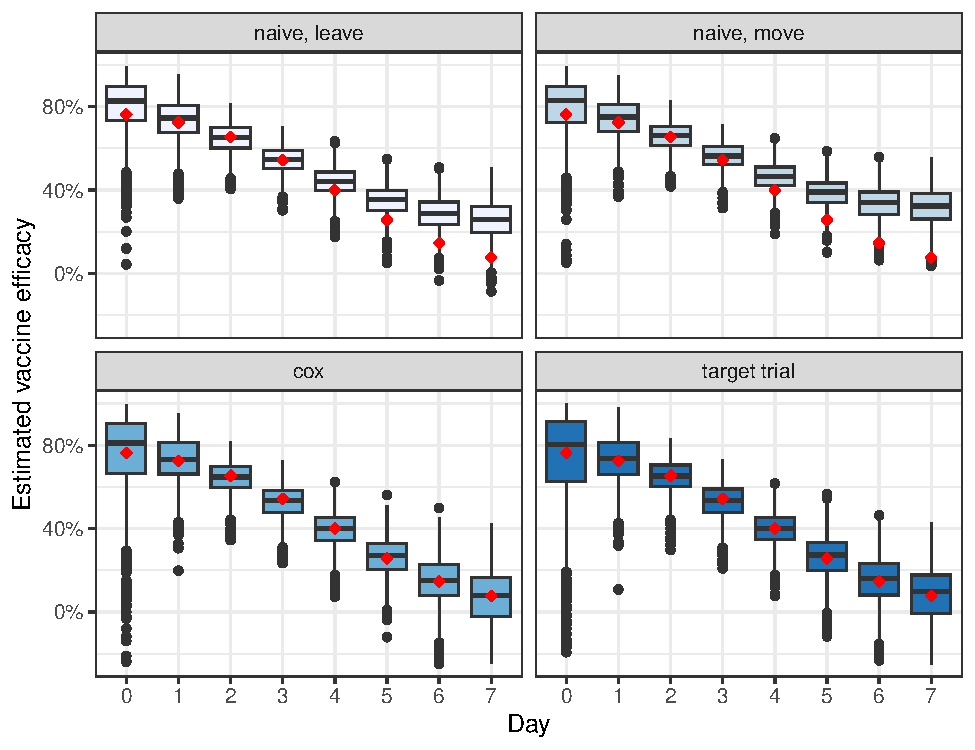
\includegraphics{../3_figures/sim_hetx.pdf}
        \caption{Comparison of estimators under when vaccine efficacy varies by postexposure administration time.\label{fig:sim_hetx}}
    \end{figure}

    \begin{figure}[p]
        \centering
        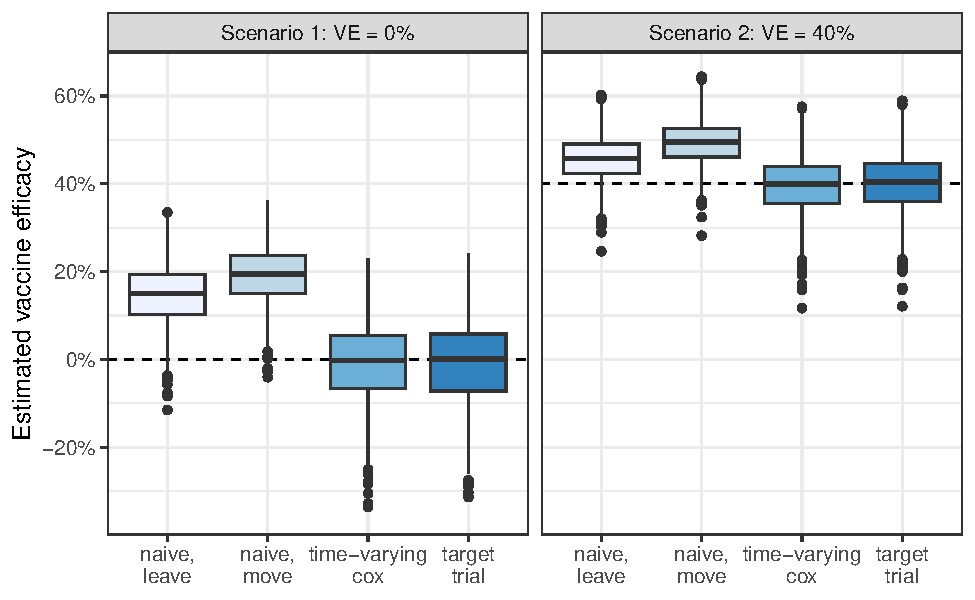
\includegraphics{../3_figures/sim_hr.pdf}
        \caption{Comparison of estimators when calculating vaccine efficacy using the hazard ratio instead of the risk ratio.\label{fig:sim_hr}}
    \end{figure}

    \begin{figure}[p]
        \centering
        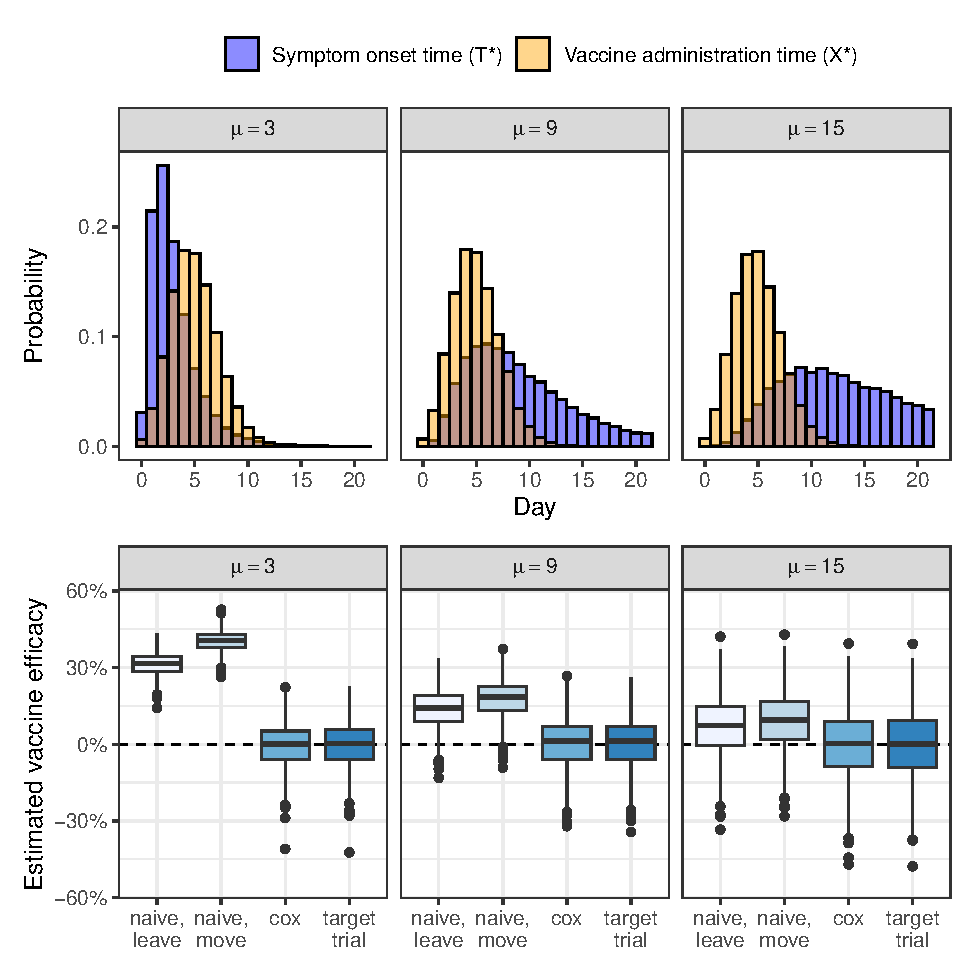
\includegraphics{../3_figures/sim_overlap.pdf}
        \caption{Bias of naive methods varies with degree of overlap between vaccination delays and symptom onset times.\label{fig:sim_overlap}}
    \end{figure}

    
    \clearpage
    % An additional complication is whether participants are screened for symptoms or PCR-positivity at enrollment and those with signs of clinical disease are excluded, in which case the regime is 
% $$
% g(X,\delta): \text{get vaccinated within $\delta$ days of exposure under }  f^*(X \mid \overline{L}_t, X > t, T > t)
% $$

% Pooled grace period:
% $$\overline{VE}_\delta = \sum_{t = 1}^\delta \left\{ 1 - \frac{\Pr[Y^{x = t} = 1]}{\Pr[Y^{x > \Delta} = 1 ]}\right\} \Pr[X = t].$$

% Pooled daily trials:

% $$\overline{VE}_\delta = \sum_{t = 1}^\delta \left\{ 1 - \frac{\Pr[Y^{x = t} = 1 \mid X = t, T > t]}{\Pr[Y^{x > \Delta} = 1 \mid X = t, T > t]}\right\} \Pr[X = t, T > t].$$

% \begin{table}[p]
%     \small
%     \centering
%     \caption{}
%     \begin{tabular}{>{\raggedright\arraybackslash}p{3cm}>{\raggedright\arraybackslash}p{4cm}>{\raggedright\arraybackslash}p{4cm}>{\raggedright\arraybackslash}p{4cm}}
%         \toprule
%         Estimand & Treatment strategies & Target trial design & Emulation \\
%         \midrule
%         $VE(0)$ & & & \\
%         $VE(t)$ & & & \\
%         $\overline{VE}_\delta$ & & & \\
%         $VE(t \mid X = t)$ & & & \\
%         \bottomrule
%     \end{tabular}
% \end{table}
% \clearpage     

    
    
\end{appendix}

\onehalfspacing

\end{document}